% The Kalman Gain, Verified: a ground-up guide to the model and its Lean proofs.
%
% Compiles with pdfLaTeX, XeLaTeX, LuaLaTeX or Tectonic; run it twice so the contents and
% cross-references settle (latexmk and Tectonic do this by themselves).
% Figures, every quoted number and the Lean excerpts are made by make_writeup_figures.py;
% build_record.txt is copied from the Lean build of Kalman.lean.
\documentclass[11pt]{article}

\usepackage[letterpaper, margin=1in]{geometry}
\usepackage{iftex}
\ifPDFTeX
  \usepackage[T1]{fontenc}
  \usepackage{lmodern}
\else
  \usepackage{fontspec}
\fi
\usepackage{amsmath, amssymb, mathtools}
\usepackage{newunicodechar}
\usepackage{graphicx}
\usepackage{xcolor}
\usepackage{booktabs, tabularx, array}
\usepackage{fancyvrb}
\usepackage{upquote}
\usepackage[skins, breakable]{tcolorbox}
\usepackage{enumitem}
\usepackage[font=small, labelfont={bf,sf}, labelsep=period]{caption}
\usepackage{titlesec}
\usepackage{parskip}
\usepackage[section]{placeins}
\usepackage[verbose=silent]{microtype}
\usepackage[hidelinks]{hyperref}
\setlength{\emergencystretch}{2.5em}

% ---------------------------------------------------------------------------------------
% Colors: the palette of the slides and the figures.
\definecolor{ink}{HTML}{0B0B0B}
\definecolor{ink2}{HTML}{52514E}
\definecolor{kblue}{HTML}{2A78D6}
\definecolor{korange}{HTML}{EB6834}
\definecolor{kaqua}{HTML}{1BAF7A}
\definecolor{wash}{HTML}{F4F3EF}

\titleformat{\section}{\normalfont\Large\sffamily\bfseries\color{ink}}{\thesection}{0.7em}{}
\titleformat{\subsection}{\normalfont\large\sffamily\bfseries\color{ink}}{\thesubsection}{0.7em}{}
\titlespacing*{\section}{0pt}{16pt}{6pt}
\titlespacing*{\subsection}{0pt}{12pt}{4pt}
\setlist{itemsep=2pt, topsep=4pt}
\renewcommand{\arraystretch}{1.25}

% Contents: sections only, as compact dotted lines. Floats: allow big figures on text pages.
\setcounter{tocdepth}{1}
\makeatletter
\renewcommand{\l@section}{\@dottedtocline{1}{0em}{1.8em}}
\makeatother
\renewcommand{\topfraction}{0.9}
\renewcommand{\bottomfraction}{0.8}
\renewcommand{\textfraction}{0.07}
\renewcommand{\floatpagefraction}{0.75}
\setcounter{topnumber}{3}
\setcounter{bottomnumber}{2}
\setcounter{totalnumber}{4}

% Numbers computed by make_writeup_figures.py, used as \val{key}.
% Generated by make_writeup_figures.py: every number the text quotes.
% kalman_writeup.tex reads them as \val{key}.
\expandafter\def\csname kfval@Pinf\endcsname{0.350}
\expandafter\def\csname kfval@PpostInf\endcsname{0.206}
\expandafter\def\csname kfval@Sinf\endcsname{0.850}
\expandafter\def\csname kfval@bK\endcsname{0.8}
\expandafter\def\csname kfval@bMean\endcsname{2.4}
\expandafter\def\csname kfval@bP\endcsname{4}
\expandafter\def\csname kfval@bR\endcsname{1}
\expandafter\def\csname kfval@bVar\endcsname{0.8}
\expandafter\def\csname kfval@bY\endcsname{3}
\expandafter\def\csname kfval@barrierHigh\endcsname{1.7}
\expandafter\def\csname kfval@barrierLow\endcsname{0.9}
\expandafter\def\csname kfval@burnThree\endcsname{35}
\expandafter\def\csname kfval@burnTwo\endcsname{24}
\expandafter\def\csname kfval@dFlag\endcsname{4}
\expandafter\def\csname kfval@dLam\endcsname{0.96}
\expandafter\def\csname kfval@dLamHat\endcsname{0.961}
\expandafter\def\csname kfval@dN\endcsname{200,000}
\expandafter\def\csname kfval@dNac\endcsname{1,000,000}
\expandafter\def\csname kfval@dRatioBad\endcsname{4.02}
\expandafter\def\csname kfval@dRatioOk\endcsname{1.00}
\expandafter\def\csname kfval@dRhoMax\endcsname{0.0029}
\expandafter\def\csname kfval@decayA\endcsname{0.72}
\expandafter\def\csname kfval@decayB\endcsname{0.72}
\expandafter\def\csname kfval@decayC\endcsname{0.75}
\expandafter\def\csname kfval@dwell\endcsname{8.6}
\expandafter\def\csname kfval@fitAsym\endcsname{6}
\expandafter\def\csname kfval@fitTrans\endcsname{2,327}
\expandafter\def\csname kfval@flowAB\endcsname{1.20}
\expandafter\def\csname kfval@flowAC\endcsname{1.64}
\expandafter\def\csname kfval@flowBA\endcsname{1.14}
\expandafter\def\csname kfval@flowBC\endcsname{1.84}
\expandafter\def\csname kfval@flowCA\endcsname{1.70}
\expandafter\def\csname kfval@flowCB\endcsname{1.79}
\expandafter\def\csname kfval@frameDt\endcsname{0.08}
\expandafter\def\csname kfval@frames\endcsname{6,250}
\expandafter\def\csname kfval@gainInf\endcsname{0.412}
\expandafter\def\csname kfval@hAlpha\endcsname{0.101}
\expandafter\def\csname kfval@hLam\endcsname{0.96}
\expandafter\def\csname kfval@hP\endcsname{0.02}
\expandafter\def\csname kfval@hRatio\endcsname{0.9600}
\expandafter\def\csname kfval@hops\endcsname{2,327}
\expandafter\def\csname kfval@mFlowAB\endcsname{0.548}
\expandafter\def\csname kfval@mFlowAC\endcsname{0.506}
\expandafter\def\csname kfval@mFlowBC\endcsname{0.355}
\expandafter\def\csname kfval@mJumps\endcsname{200,000}
\expandafter\def\csname kfval@mKappaAB\endcsname{1.416}
\expandafter\def\csname kfval@mKappaAC\endcsname{1.599}
\expandafter\def\csname kfval@mKappaBC\endcsname{1.449}
\expandafter\def\csname kfval@mOcc\endcsname{0.501, 0.300, 0.199}
\expandafter\def\csname kfval@mOccErr\endcsname{0.001}
\expandafter\def\csname kfval@mRateAB\endcsname{1.097}
\expandafter\def\csname kfval@mRateAC\endcsname{1.011}
\expandafter\def\csname kfval@mRateBA\endcsname{1.828}
\expandafter\def\csname kfval@mRateBC\endcsname{1.183}
\expandafter\def\csname kfval@mRateCA\endcsname{2.528}
\expandafter\def\csname kfval@mRateCB\endcsname{1.774}
\expandafter\def\csname kfval@mRes\endcsname{6\times 10^{-17}}
\expandafter\def\csname kfval@molPhi\endcsname{62}
\expandafter\def\csname kfval@nDefsCore\endcsname{3}
\expandafter\def\csname kfval@nDefsModel\endcsname{11}
\expandafter\def\csname kfval@nProofs\endcsname{38}
\expandafter\def\csname kfval@nSpec\endcsname{17}
\expandafter\def\csname kfval@occA\endcsname{0.47}
\expandafter\def\csname kfval@occB\endcsname{0.31}
\expandafter\def\csname kfval@occC\endcsname{0.22}
\expandafter\def\csname kfval@occRunA\endcsname{0.47}
\expandafter\def\csname kfval@occRunB\endcsname{0.32}
\expandafter\def\csname kfval@occRunC\endcsname{0.21}
\expandafter\def\csname kfval@ouA\endcsname{0.905}
\expandafter\def\csname kfval@ouStart\endcsname{2.4}
\expandafter\def\csname kfval@ouTau\endcsname{10}
\expandafter\def\csname kfval@popA\endcsname{0.49}
\expandafter\def\csname kfval@popB\endcsname{0.30}
\expandafter\def\csname kfval@popC\endcsname{0.21}
\expandafter\def\csname kfval@rAsq\endcsname{0.819}
\expandafter\def\csname kfval@rSlope\endcsname{0.283}
\expandafter\def\csname kfval@rWorst\endcsname{0.59}
\expandafter\def\csname kfval@relax\endcsname{0.25}
\expandafter\def\csname kfval@runA\endcsname{0.905}
\expandafter\def\csname kfval@runIn\endcsname{78}
\expandafter\def\csname kfval@runLate\endcsname{80}
\expandafter\def\csname kfval@runPzero\endcsname{5}
\expandafter\def\csname kfval@runQ\endcsname{0.181}
\expandafter\def\csname kfval@runR\endcsname{0.5}
\expandafter\def\csname kfval@sigmaSqA\endcsname{0.12}
\expandafter\def\csname kfval@sigmaSqB\endcsname{0.12}
\expandafter\def\csname kfval@sigmaSqC\endcsname{0.13}
\expandafter\def\csname kfval@theta\endcsname{0.5}
\expandafter\def\csname kfval@thrH\endcsname{0.013}
\expandafter\def\csname kfval@thrK\endcsname{0.13}
\expandafter\def\csname kfval@walkers\endcsname{40}

\DeclareRobustCommand{\val}[1]{\ifcsname kfval@#1\endcsname\csname kfval@#1\endcsname%
  \else\textbf{??}\PackageWarning{kalman}{No number named #1}\fi}

% How the non-ASCII characters of the Lean excerpts are typeset.
% Generated by make_writeup_figures.py: how the Lean excerpts' non-ASCII
% characters are typeset (loaded by kalman_writeup.tex).
\newunicodechar{²}{\ensuremath{^{2}}}
\newunicodechar{·}{\ensuremath{\cdot}}
\newunicodechar{Ω}{\ensuremath{\Omega}}
\newunicodechar{α}{\ensuremath{\alpha}}
\newunicodechar{β}{\ensuremath{\beta}}
\newunicodechar{κ}{\ensuremath{\kappa}}
\newunicodechar{μ}{\ensuremath{\mu}}
\newunicodechar{σ}{\ensuremath{\sigma}}
\newunicodechar{τ}{\ensuremath{\tau}}
\newunicodechar{ω}{\ensuremath{\omega}}
\newunicodechar{ᵀ}{\ensuremath{^{\mathsf{T}}}}
\newunicodechar{ᵢ}{\ensuremath{_{i}}}
\newunicodechar{•}{\ensuremath{\bullet}}
\newunicodechar{ⁿ}{\ensuremath{^{n}}}
\newunicodechar{₀}{\ensuremath{_{0}}}
\newunicodechar{₁}{\ensuremath{_{1}}}
\newunicodechar{₂}{\ensuremath{_{2}}}
\newunicodechar{ℕ}{\ensuremath{\mathbb{N}}}
\newunicodechar{ℝ}{\ensuremath{\mathbb{R}}}
\newunicodechar{←}{\ensuremath{\leftarrow}}
\newunicodechar{→}{\ensuremath{\to}}
\newunicodechar{↔}{\ensuremath{\leftrightarrow}}
\newunicodechar{∀}{\ensuremath{\forall}}
\newunicodechar{∈}{\ensuremath{\in}}
\newunicodechar{∑}{\ensuremath{\textstyle\sum}}
\newunicodechar{√}{\ensuremath{\surd}}
\newunicodechar{∧}{\ensuremath{\land}}
\newunicodechar{≠}{\ensuremath{\ne}}
\newunicodechar{≤}{\ensuremath{\le}}
\newunicodechar{⟂}{\ensuremath{\perp}}
\newunicodechar{ⱼ}{\ensuremath{_{j}}}
\newunicodechar{𝓝}{\ensuremath{\mathcal{N}}}


% Lean code: a verbatim excerpt of Kalman.lean, or a short inline fragment.
\newcommand{\leancodesize}{\fontsize{8}{9.8}\selectfont}
\newcommand{\leanfile}[1]{%
  \begin{tcolorbox}[enhanced, breakable, colback=wash, colframe=wash, boxrule=0pt, arc=2pt,
      left=4pt, right=4pt, top=2pt, bottom=2pt, before skip=6pt, after skip=6pt]%
    \VerbatimInput[fontsize=\leancodesize]{generated/lean/#1.lean}%
  \end{tcolorbox}}
\newcommand{\leanus}{\textunderscore\allowbreak}% long Lean names may break after an underscore
\newcommand{\lean}[1]{\begingroup\let\_\leanus\texttt{#1}\endgroup}

% Boxes.
\newtcolorbox{keybox}[1]{enhanced, breakable, colback=kblue!4, colframe=kblue!70,
  boxrule=0.5pt, arc=2pt, left=7pt, right=7pt, top=4pt, bottom=4pt,
  fonttitle=\sffamily\bfseries\small, coltitle=ink, colbacktitle=kblue!14, title={#1},
  before skip=8pt, after skip=8pt}
\newtcolorbox{intuitionbox}{enhanced, breakable, frame hidden, sharp corners,
  colback=korange!6, borderline west={2.2pt}{0pt}{korange}, left=8pt, right=6pt, top=3pt,
  bottom=3pt, before skip=8pt, after skip=10pt}
\newcommand{\intuition}[1]{\begin{intuitionbox}\textsf{\textbf{Intuition:}}\ \textit{#1}%
  \end{intuitionbox}}
\newcommand{\reads}[2]{%
  \begin{tcolorbox}[enhanced, breakable, frame hidden, sharp corners, colback=white,
      borderline west={1.6pt}{0pt}{kaqua}, left=8pt, right=4pt, top=1pt, bottom=1pt,
      before skip=2pt, after skip=10pt]
    \textsf{\textbf{In words:}} #1\par\smallskip
    \textsf{\textbf{For the model:}} #2
  \end{tcolorbox}}

% A part heading that is not LaTeX's \part (kept simple and engine independent).
\newcommand{\partheading}[2]{%
  \clearpage
  \phantomsection
  \addcontentsline{toc}{part}{\texorpdfstring{Part #1\quad #2}{Part #1: #2}}%
  \begin{tcolorbox}[enhanced, colback=wash, colframe=wash, arc=2pt, left=10pt, right=10pt,
      top=8pt, bottom=8pt, after skip=10pt]
    {\sffamily\small\color{ink2}PART #1}\par\vspace{2pt}
    {\sffamily\bfseries\LARGE\color{ink}#2}
  \end{tcolorbox}}

\newcommand{\Var}{\operatorname{Var}}
\newcommand{\Ex}{\mathbb{E}}
\newcommand{\RR}{\mathbb{R}}
\newcommand{\transp}{\mathsf{T}}
\newcommand{\postVar}{\mathrm{postVar}}
\newcommand{\optVar}{\mathrm{optVar}}
\newcommand{\figwidth}{\linewidth}

\hypersetup{pdftitle={The Kalman Gain, Verified}, pdfauthor={Jeffrey Lee}}

\begin{document}

% =======================================================================================
\begin{center}
  {\sffamily\bfseries\Huge\color{ink}The Kalman Gain, Verified\par}
  \vspace{6pt}
  {\large A ground-up guide to a molecular switching model,\\
    what it should satisfy, and how Lean proves it\par}
  \vspace{8pt}
  {\sffamily\color{ink2}Jeffrey Lee\quad\textperiodcentered\quad
    Brown CS 1715, Formal Proof and Verification\quad\textperiodcentered\quad November 2026\par}
\end{center}

\begin{keybox}{At a glance}
  \begin{itemize}[leftmargin=1.2em]
    \item \textbf{What.} A simple model of how a molecule moves (a \emph{switching diffusion}),
      a filter that tracks it from noisy measurements (the \emph{Kalman filter}), and
      \val{nSpec} facts about both, proved in the proof assistant Lean~4 with its mathematics
      library Mathlib.
    \item \textbf{Who it is for.} Anyone who knows calculus, a little linear algebra and a
      little probability. No physics or chemistry is assumed.
    \item \textbf{How to read it.} Part~I builds the model from scratch. Part~II says what is
      worth proving about it and what the proofs assume. Part~III shows how the model is
      defined in Lean and how the theorems are stated. Appendix~A sketches every proof.
      Each section ends with a one-line \emph{intuition}.
  \end{itemize}
\end{keybox}

\begin{figure}[h]
  \centering
  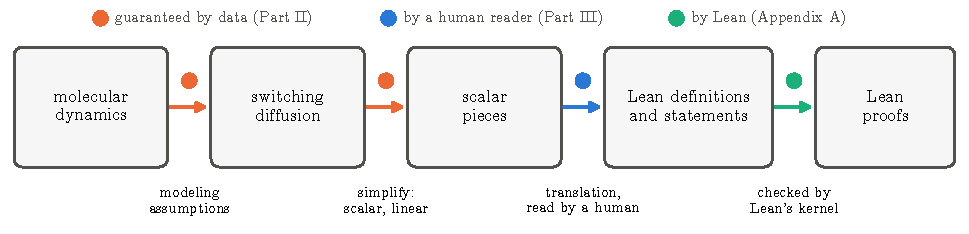
\includegraphics[width=\figwidth]{figures/ladder.pdf}
  \caption{The road from a real molecule to a checked theorem. The first two steps are
    modeling choices that only data can support (Part~II); the third is a translation that a
    person must read (Part~III); the last is checked by Lean (Appendix~A).}
  \label{fig:ladder}
\end{figure}

{\small\tableofcontents}

% =======================================================================================
\partheading{I}{The model, from the ground up}

\section{A molecule is a point that moves}

A molecule is a handful of atoms, from a few to many thousands. Each atom sits at a point in
space, given by three numbers, so a molecule with $N$ atoms is described by $3N$ numbers.
Listing them gives one point
\[
  x = (x_1, y_1, z_1, \dots, x_N, y_N, z_N) \in \RR^{3N},
\]
called the \emph{configuration}. As the atoms jiggle, $x$ moves. A \emph{molecular dynamics}
(MD) simulation is a program that computes this motion and saves a snapshot of $x$ every
$\Delta t$; each snapshot is a \emph{frame}.

Nobody looks at all $3N$ numbers. We look at \emph{coordinates}: real-valued functions of $x$
that describe the shape, such as the distance between two atoms, or the \emph{torsion}
$\varphi$, the twist about the bond between atoms 2 and~3 (Figure~\ref{fig:molecule}).
Precisely, $\varphi$ is the angle between the plane through atoms 1, 2, 3 and the plane
through atoms 2, 3, 4. A \emph{coordinate family} is a group of similar coordinates, for
example all the backbone torsions of a protein.

\begin{figure}[htbp]
  \centering
  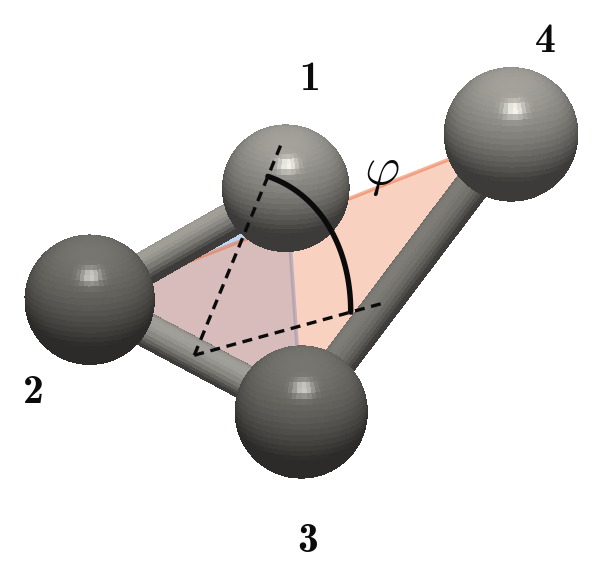
\includegraphics[width=0.42\linewidth]{figures/molecule.png}
  \caption{Four atoms joined by three bonds. The torsion $\varphi$ is the angle between the
    blue triangle (atoms 1, 2, 3) and the orange one (atoms 2, 3, 4), measured about the bond
    2--3; here $\varphi = \val{molPhi}^\circ$. The configuration of these four atoms is one
    point of $\RR^{12}$, and $\varphi$ is a function of that point.}
  \label{fig:molecule}
\end{figure}

\intuition{a molecule is a moving point in a space of many dimensions; a coordinate is a
  function of that point.}

\section{The energy landscape}

Every configuration $x$ has an \emph{energy} $V(x)$, a real number computed from the atom
positions. One fact about it is enough here: low energy means a comfortable shape. So think of
$V\colon \RR^{3N} \to \RR$ as a landscape. Its valleys are the stable shapes, called
\emph{basins}; the mountain passes between valleys are the routes from one shape to another.

\begin{keybox}{Definition (basin)}
  Let $c_1, \dots, c_n$ be the local minima of $V$. The \emph{basin} of $c_i$ is the set of
  starting points from which steepest descent, $\dot x = -\nabla V(x)$, ends at $c_i$.
\end{keybox}

Since $\RR^{3N}$ cannot be drawn, Figure~\ref{fig:landscape} shows a toy landscape over a plane,
with three basins called A, B and C. The same toy is used throughout Part~I.

\begin{figure}[htbp]
  \centering
  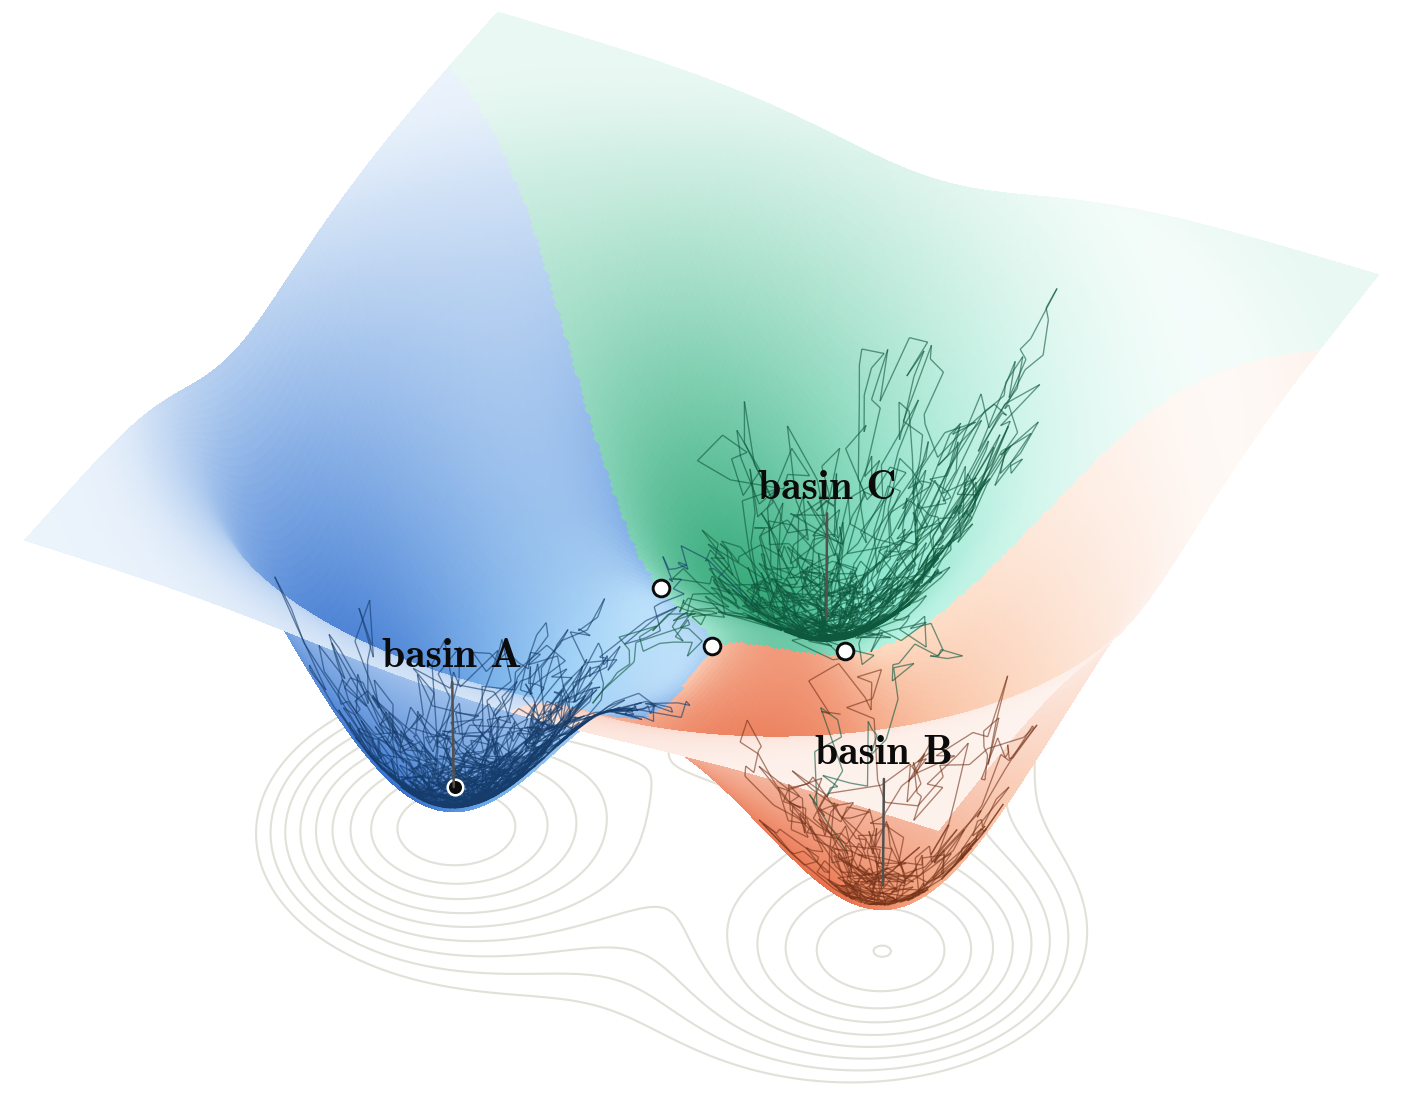
\includegraphics[width=0.86\linewidth]{figures/landscape.png}
  \caption{A toy energy landscape $V(x_1, x_2)$ with three basins (blue A, orange B,
    green C); white dots mark the passes. The dark path is a simulated motion
    (Section~\ref{sec:motion}): it rattles inside a basin and now and then crosses a pass. The
    passes lie \val{barrierLow} to \val{barrierHigh} energy units above the valley floors.}
  \label{fig:landscape}
\end{figure}

\intuition{valleys are shapes the molecule likes; passes are the ways between them.}

\section{How the molecule moves: downhill plus random kicks}\label{sec:motion}

A standard simplified model of MD motion is gradient descent with noise:
\begin{equation}\label{eq:langevin}
  x_{k+1} = x_k - \nabla V(x_k)\,\Delta t + \sqrt{2\theta\,\Delta t}\;\xi_k,
  \qquad \xi_k \sim \mathcal N(0, I) \text{ independent}.
\end{equation}
The first term pulls $x$ downhill; the second adds a random kick whose size is set by
$\theta > 0$ (physicists call $\theta$ the temperature; the toy uses $\theta = \val{theta}$).
This is the overdamped Langevin equation, taken in small time steps.

Two time scales appear (Figure~\ref{fig:timescales}a).
\begin{itemize}
  \item \textbf{Fast:} inside a basin, pull and kicks balance, and $x$ rattles about the
    bottom. In the toy, the rattle forgets itself in about \val{relax} time units.
  \item \textbf{Slow:} now and then a lucky run of kicks carries $x$ over a pass, and it
    starts rattling in another basin. Hops are rare because they need many kicks in the same
    direction; in the toy, a stay in one basin lasts \val{dwell} time units on average.
\end{itemize}

\begin{figure}[htbp]
  \centering
  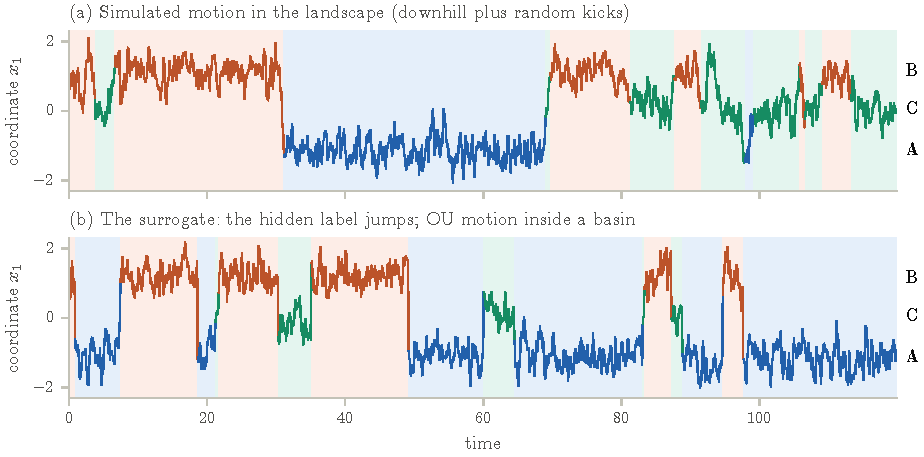
\includegraphics[width=\figwidth]{figures/timescales.pdf}
  \caption{(a) The coordinate $x_1$ of one simulated run of \eqref{eq:langevin}, colored by
    basin: fast rattling, rare hops. (b) The surrogate model of Section~\ref{sec:surrogate},
    with its parameters read off the simulated runs (\val{walkers} runs of \val{frames} frames,
    \val{fitTrans} hops in all). It reproduces both time scales with far simpler mechanics.}
  \label{fig:timescales}
\end{figure}

\intuition{a fast rattle inside a basin and rare hops between basins: two very different
  clocks.}

\section{Equilibrium: where the molecule spends its time}\label{sec:equilibrium}

Run \eqref{eq:langevin} for a long time and record where $x$ is. For a long run and a small
$\Delta t$, the fraction of time spent in a region $A$ is close to $\int_A \pi(x)\,dx$, where
\begin{equation}\label{eq:boltzmann}
  \pi(x) = \frac{e^{-V(x)/\theta}}{Z}, \qquad Z = \int e^{-V(x)/\theta}\,dx .
\end{equation}
This is the \emph{Boltzmann distribution}; we take it as a known fact about
\eqref{eq:langevin}. Deep valleys get exponentially more time. The \emph{population} of basin
$i$ is $p_i = \int_{\text{basin } i} \pi(x)\,dx$, its long-run share of time
(Figure~\ref{fig:density}). In the toy, $p_A = \val{popA}$, $p_B = \val{popB}$ and
$p_C = \val{popC}$.

The equilibrium is also \emph{reversible}: a long equilibrium movie looks statistically the
same played backwards. In particular, hops from $i$ to $j$ happen as often as hops from $j$ to
$i$. In the simulated runs the measured flows of each pair agree to within \val{fitAsym}\%,
which is sampling noise. A simplified model should keep both features, the populations and the
balanced flows. That is result~M of Part~III.

\begin{figure}[htbp]
  \centering
  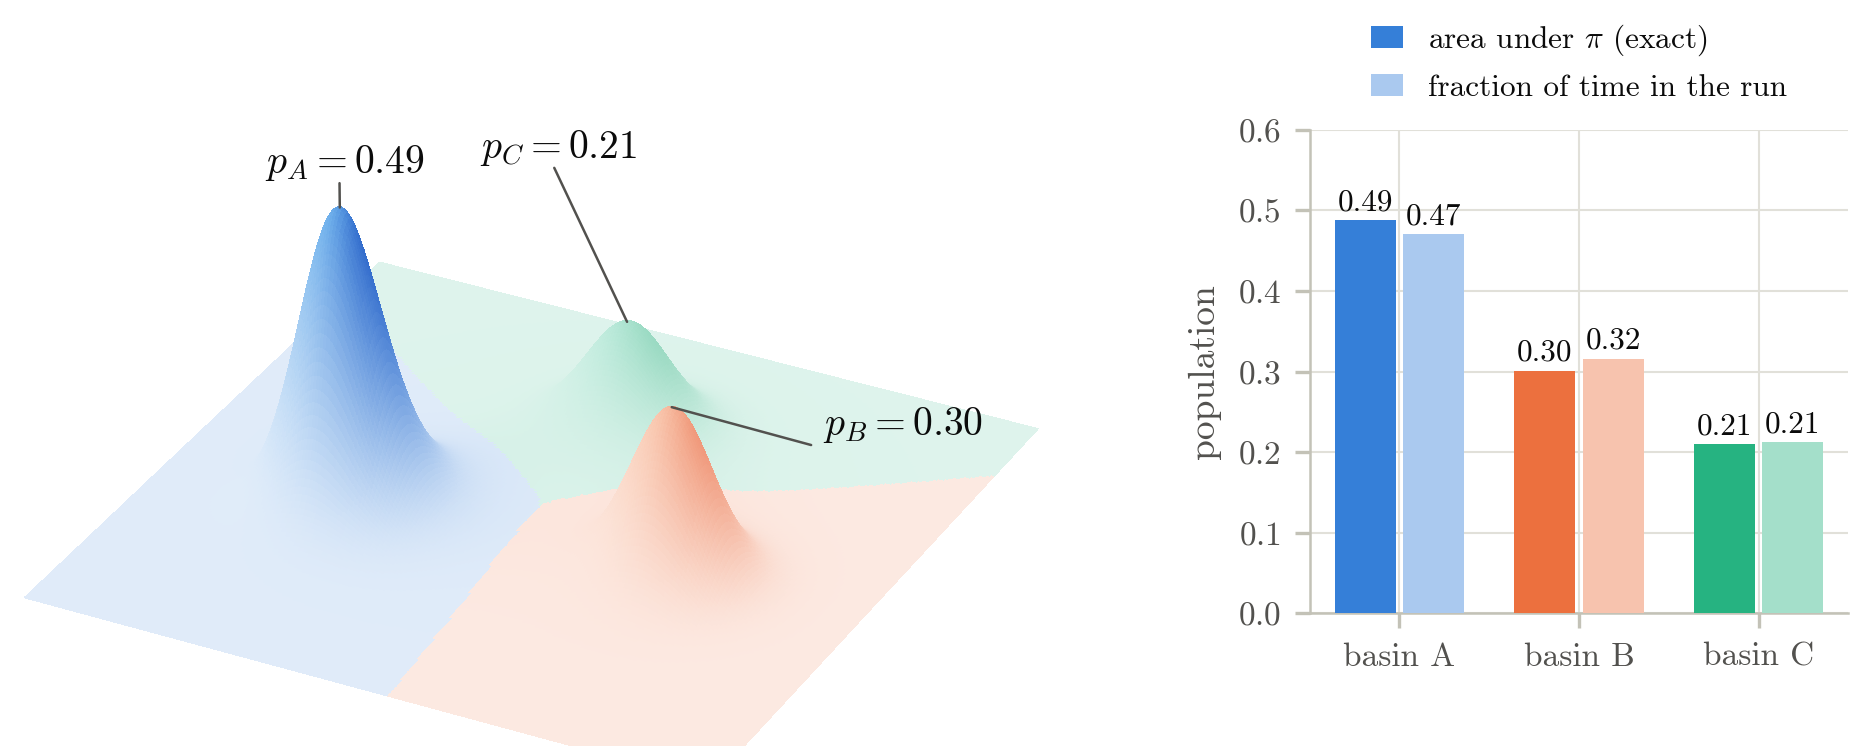
\includegraphics[width=\figwidth]{figures/density.png}
  \caption{Left: the equilibrium density $\pi$ of \eqref{eq:boltzmann} for the toy landscape,
    colored by basin, with each basin's population. Right: the populations (exact, from
    $\pi$) against the fraction of time the simulated runs spent in each basin.}
  \label{fig:density}
\end{figure}

\intuition{in the long run, the time spent near a shape is proportional to
  $e^{-\text{energy}/\theta}$.}

\section{The surrogate: a switching diffusion}\label{sec:surrogate}

MD is expensive and lives in thousands of dimensions. The research model replaces it by two
simple pieces (Figure~\ref{fig:switching}).
\begin{enumerate}
  \item A hidden \emph{basin label} $s_t \in \{1, \dots, n\}$ that jumps between basins at
    random times. From basin $i$ it jumps to basin $j$ at \emph{rate} $k_{ij}$: in a short time
    $dt$ the jump happens with probability about $k_{ij}\,dt$.
  \item Inside the current basin, the slow coordinates follow an \emph{Ornstein--Uhlenbeck}
    (OU) process: pulled back toward the basin's center and kicked at random
    (Section~\ref{sec:ou}).
\end{enumerate}
A diffusion whose rules switch with a hidden label is a \emph{switching diffusion}. It keeps
the two clocks of Section~\ref{sec:motion}: OU rattle inside a basin, jumps between basins.

\textbf{The jump rule.} With the slow coordinates held fixed, the research model uses
\begin{equation}\label{eq:jump}
  k_{ij} = \kappa_{ij}\sqrt{p_j / p_i}, \qquad \kappa_{ij} = \kappa_{ji} > 0 .
\end{equation}
Here $\kappa_{ij}$ is a symmetric attempt rate for the pair $\{i, j\}$. The square root speeds
up jumps toward the more populated basin and slows the reverse by the same factor. Writing
$p_i \propto e^{-V_i/\theta}$ gives $k_{ij} = \kappa_{ij}\,e^{-(V_j - V_i)/2\theta}$: the energy
difference is split evenly between the two directions. (Rates of this form are known in the
MD literature as the square-root approximation.) In the full model $p_i$ and $\kappa_{ij}$ may
depend on the slow coordinates; result~M is about one fixed value of them.

\textbf{The generator.} Collect the rates in a matrix $L$ with $L_{ij} = k_{ij}$ for
$i \ne j$ and $L_{ii} = -\sum_{j \ne i} k_{ij}$, so that every row sums to $0$. If $q(t)$ is
the row vector of probabilities of the label at time $t$, then $\tfrac{d}{dt}\,q(t) = q(t)\,L$.
A population vector $p$ is \emph{stationary} when $p^\transp L = 0$: started at $p$, the
probabilities never change. Figure~\ref{fig:threebasins} shows a three-basin example.

\begin{figure}[htbp]
  \centering
  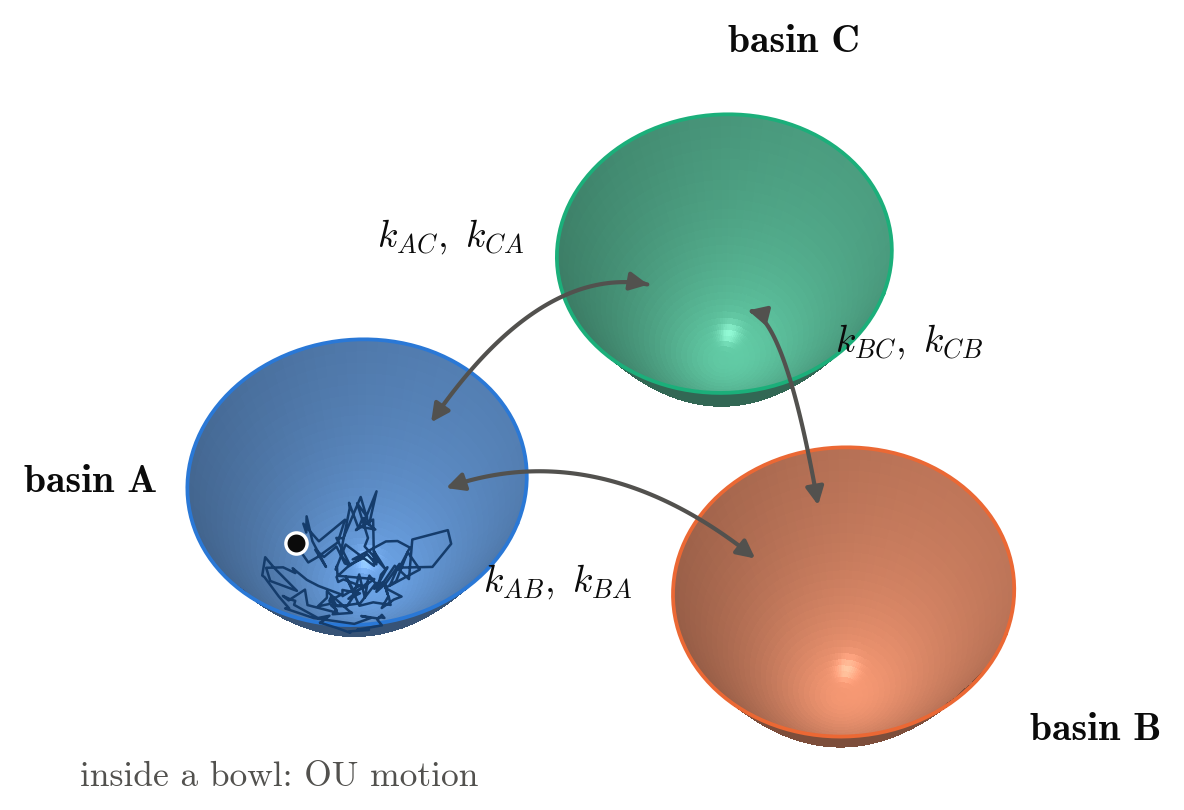
\includegraphics[width=0.74\linewidth]{figures/switching.png}
  \caption{The switching diffusion. Each basin becomes a quadratic bowl in which the slow
    coordinates follow OU motion (dark path and ball); the hidden label jumps between bowls at
    rates $k_{ij}$. Fitted to the toy runs, the bowls have equilibrium variances
    \val{sigmaSqA}, \val{sigmaSqB}, \val{sigmaSqC} in $x_1$ and per-frame decays
    \val{decayA}, \val{decayB}, \val{decayC}.}
  \label{fig:switching}
\end{figure}

\begin{figure}[htbp]
  \centering
  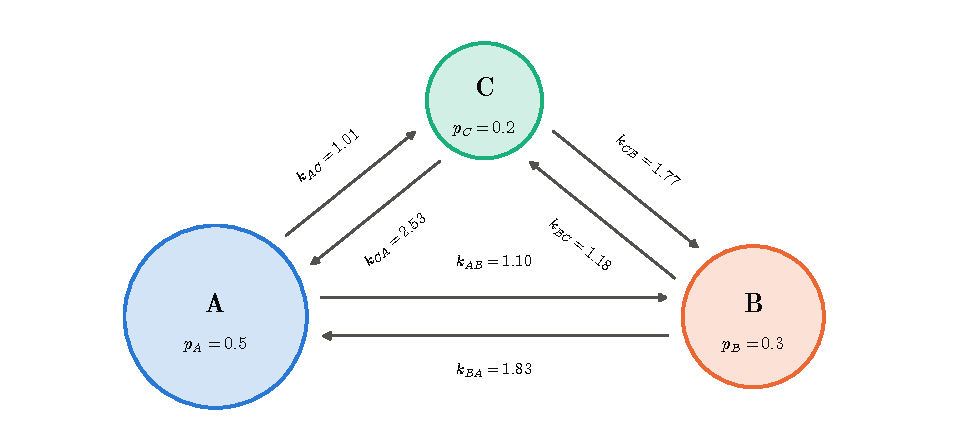
\includegraphics[width=0.9\linewidth]{figures/three_basins.pdf}
  \caption{The jump rule \eqref{eq:jump} for populations $p = (0.5, 0.3, 0.2)$ and random
    symmetric prefactors ($\kappa_{AB} = \val{mKappaAB}$, $\kappa_{AC} = \val{mKappaAC}$,
    $\kappa_{BC} = \val{mKappaBC}$). Each pair trades equal flows both ways:
    $p_A k_{AB} = p_B k_{BA} = \val{mFlowAB}$, $p_A k_{AC} = p_C k_{CA} = \val{mFlowAC}$ and
    $p_B k_{BC} = p_C k_{CB} = \val{mFlowBC}$. In floating point the largest entry of
    $|p^\transp L|$ is $\val{mRes}$, and \val{mJumps} simulated jumps occupy the basins in
    proportions \val{mOcc}.}
  \label{fig:threebasins}
\end{figure}

\intuition{replace the landscape by bowls, and the passes by a weighted coin flip.}

\section{Inside one basin: the Ornstein--Uhlenbeck process}\label{sec:ou}

Near the bottom $c$ of a valley, $V$ is close to a parabola. In one coordinate,
$V(x) \approx V(c) + \tfrac{k}{2}(x - c)^2$, so the pull $-V'(x) = -k(x - c)$ is linear in the
distance from the bottom. A process pulled back linearly and kicked at random is an OU
process. Sampled every $\Delta t$ and shifted so that the center is $0$, it obeys exactly
\begin{equation}\label{eq:ou}
  z_{n+1} = a\,z_n + w_n, \qquad w_n \sim \mathcal N(0, Q), \qquad
  a = e^{-\Delta t/\tau_c}, \quad Q = \sigma^2 (1 - a^2),
\end{equation}
with independent $w_n$. Here $\tau_c$ is the \emph{relaxation time} and $\sigma^2$ the
\emph{equilibrium variance}. For \eqref{eq:langevin}, $\tau_c = 1/k$ and $\sigma^2 = \theta/k$:
a flat basin (small $k$) is wide and slow.

Two consequences follow by induction on $n$:
\[
  \Ex[z_n] = a^n\,\Ex[z_0], \qquad \Var(z_n) = a^{2n}\Var(z_0) + \sigma^2(1 - a^{2n}).
\]
The mean forgets the start by a factor $a$ per frame, and the variance tends to $\sigma^2$
(Figure~\ref{fig:ou}). The rule that pushes a variance $P$ through one step,
\[
  P \;\mapsto\; a^2 P + \sigma^2(1 - a^2),
\]
is the Lean definition \lean{ouPredict}. It leaves $\sigma^2$ unchanged: if
$\Var(z_n) = \sigma^2$ then $\Var(z_{n+1}) = \sigma^2$.

\begin{figure}[htbp]
  \centering
  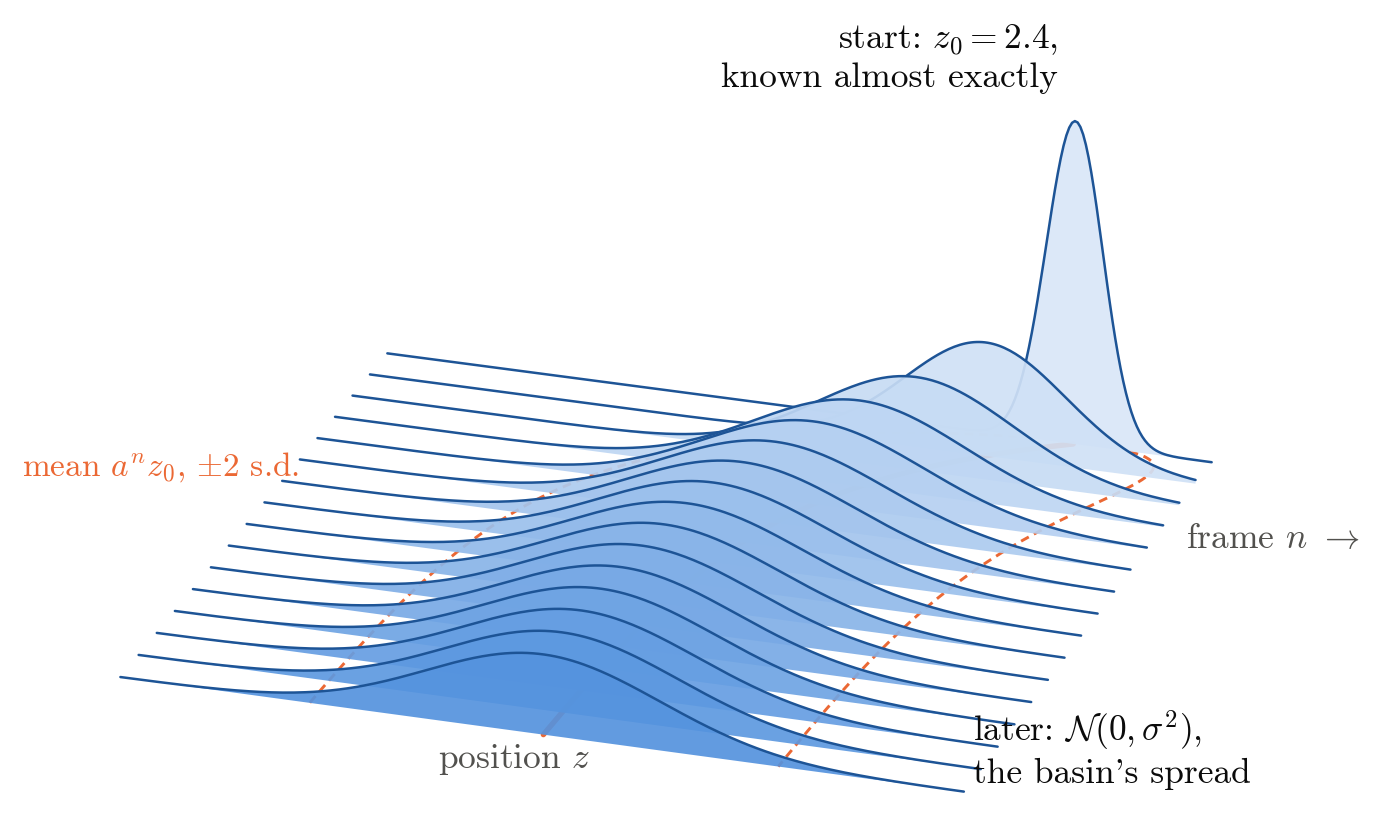
\includegraphics[width=0.84\linewidth]{figures/ou.png}
  \caption{An OU mode forgets its start. Each slice is the density of $z_n$ for a start
    $z_0 = \val{ouStart}$ known almost exactly, with relaxation time $\tau_c = \val{ouTau}$
    frames (so $a = \val{ouA}$) and $\sigma^2 = 1$. The orange lines on the floor are the mean
    $a^n z_0$ and two standard deviations either side.}
  \label{fig:ou}
\end{figure}

\intuition{inside a basin, uncertainty grows to the basin's width and stops there.}

\section{Sensors: what we actually see}

We never see the slow state directly. Each coordinate family $c$ acts as a noisy
\emph{sensor} of it:
\[
  y_c = z + v_c, \qquad v_c \sim \mathcal N(0, R_c),
\]
with $v_c$ independent of $z$, of the other sensors and of the past. The number $R_c$ is the
sensor's \emph{noise variance}. (In general a family measures a linear function $H_c z$ of a
vector of slow coordinates; the formalization treats the scalar case $H_c = 1$.)

\intuition{a slow hidden state, seen through several noisy windows.}

\section{The Kalman filter: predict, then correct}\label{sec:kalman}

The filter keeps a best guess $m$ of the hidden state and the variance $P$ of its error.
Figure~\ref{fig:frame} shows what happens in one frame.

\begin{figure}[htbp]
  \centering
  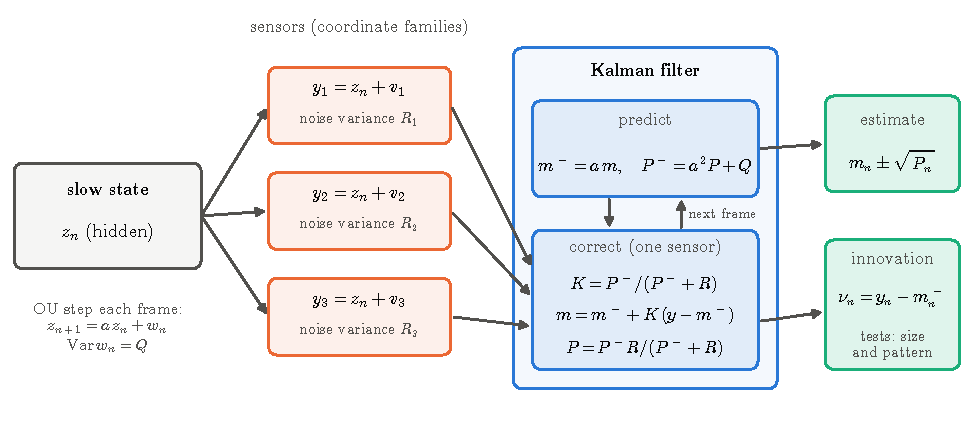
\includegraphics[width=\figwidth]{figures/frame.pdf}
  \caption{One frame. The hidden state takes an OU step; each sensor reports it with its own
    noise; the filter predicts, then corrects with each reading; it outputs an estimate with
    its uncertainty, and an innovation for each reading (Section~\ref{sec:innovations}).}
  \label{fig:frame}
\end{figure}

\subsection*{Correct: the navigator and the lookout}

Think of a ship's navigator, whose prediction $m^-$ of the position misses the truth by
$e = z - m^-$ with $\Var(e) = P$, and a lookout, whose sighting $y = z + v$ misses by $v$ with
$\Var(v) = R$, independent of $e$. Blend the two with a \emph{gain} $K \in \RR$:
\[
  m = m^- + K\,(y - m^-).
\]
$K = 0$ ignores the sighting and $K = 1$ ignores the prediction. The new error is
$z - m = (1 - K)\,e - K\,v$. Two rules give its variance: $\Var(cX) = c^2 \Var(X)$, and
$\Var(X + Y) = \Var(X) + \Var(Y)$ when $X$ and $Y$ are independent. Hence
\begin{equation}\label{eq:postvar}
  \Var(z - m) = (1 - K)^2 P + K^2 R \;=\; \postVar(P, R, K).
\end{equation}
Which gain is best? Completing the square in $K$ (using $P + R > 0$):
\begin{equation}\label{eq:square}
  \postVar(P, R, K) = (P + R)\,(K - K^*)^2 + \frac{PR}{P + R},
  \qquad K^* = \frac{P}{P + R}.
\end{equation}
The square is never negative and vanishes only at $K = K^*$. So $K^*$, the \emph{Kalman
gain}, is the unique best gain, and the smallest variance is
\[
  \optVar(P, R) = \frac{PR}{P + R}, \qquad\text{equivalently}\qquad
  \frac{1}{\optVar(P, R)} = \frac{1}{P} + \frac{1}{R}.
\]
Precisions (one over variance) add. In particular $\optVar \le P$ and $\optVar \le R$: the
blend beats both sources. Figure~\ref{fig:bayes} gives a second view. For Gaussian errors,
reading $y$ slices the joint density of state and reading, and the slice is exactly the
updated belief $\mathcal N(m, \optVar)$. Figure~\ref{fig:valley} draws \eqref{eq:square} as a
valley whose floor is the Kalman gain.

\begin{figure}[htbp]
  \centering
  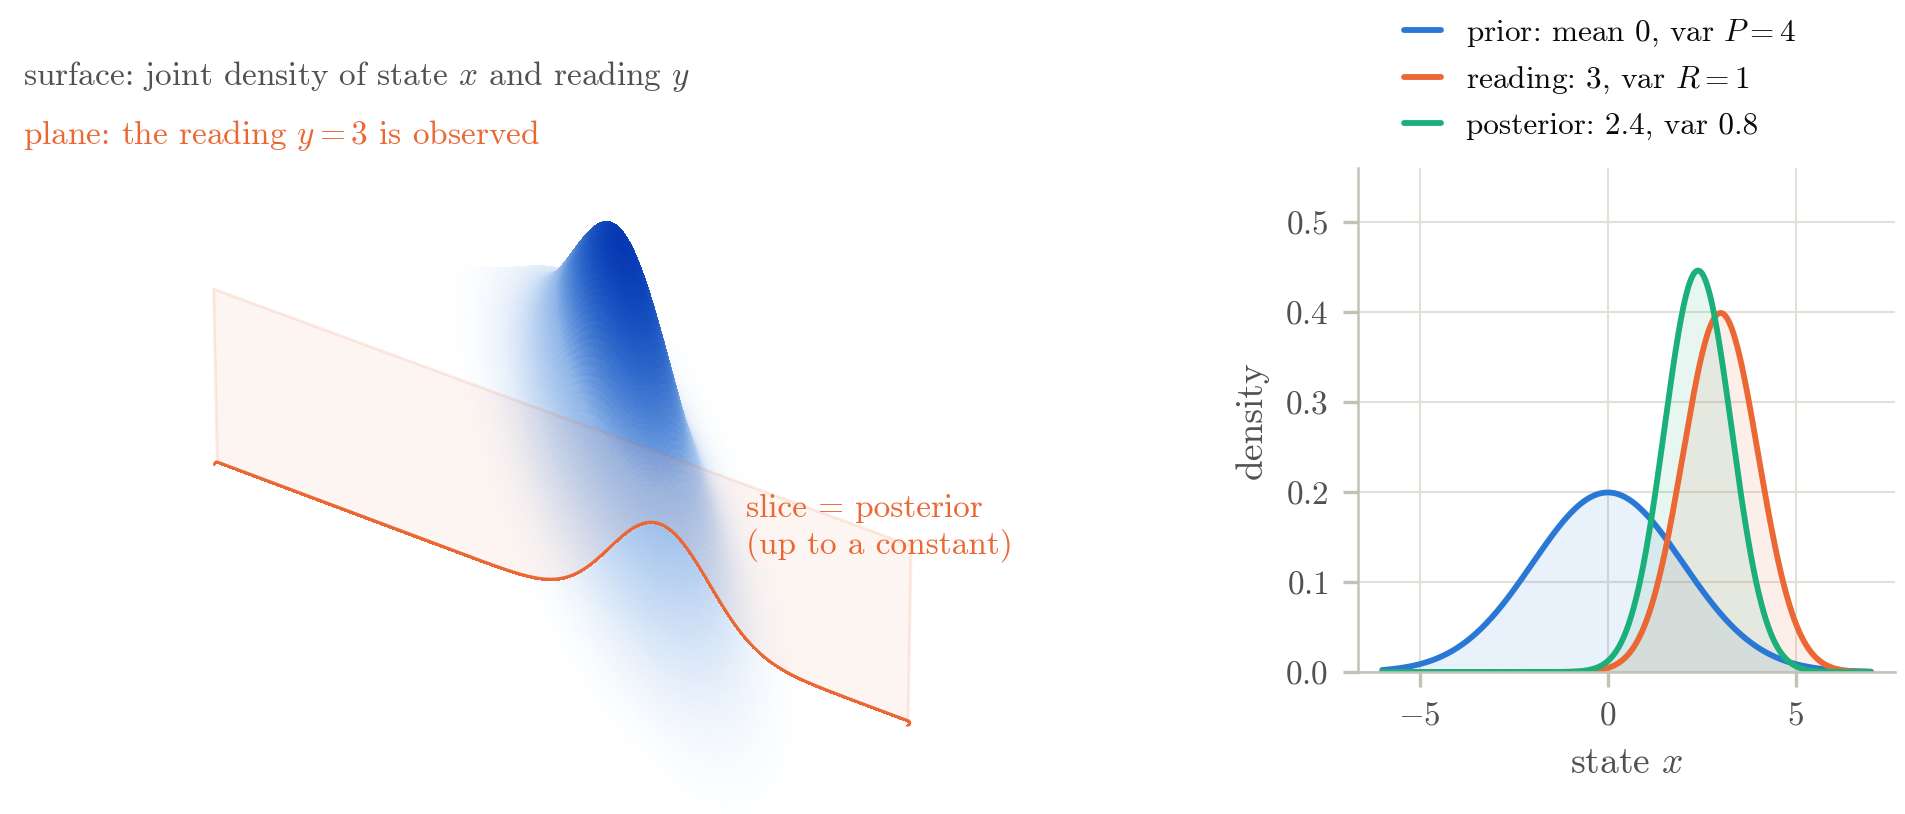
\includegraphics[width=\figwidth]{figures/bayes.png}
  \caption{The update as a slice. Prior $\mathcal N(0, \val{bP})$, reading noise variance
    $\val{bR}$, reading $y = \val{bY}$. Left: the joint density of state and reading; the
    orange curve is its slice at $y = \val{bY}$. Right: that slice, normalized, is the
    posterior, with mean $\val{bK} \cdot \val{bY} = \val{bMean}$ (gain $K^* = \val{bK}$) and
    variance $\val{bP} \cdot \val{bR} / (\val{bP} + \val{bR}) = \val{bVar}$, narrower than the
    prior and than the reading.}
  \label{fig:bayes}
\end{figure}

\begin{figure}[htbp]
  \centering
  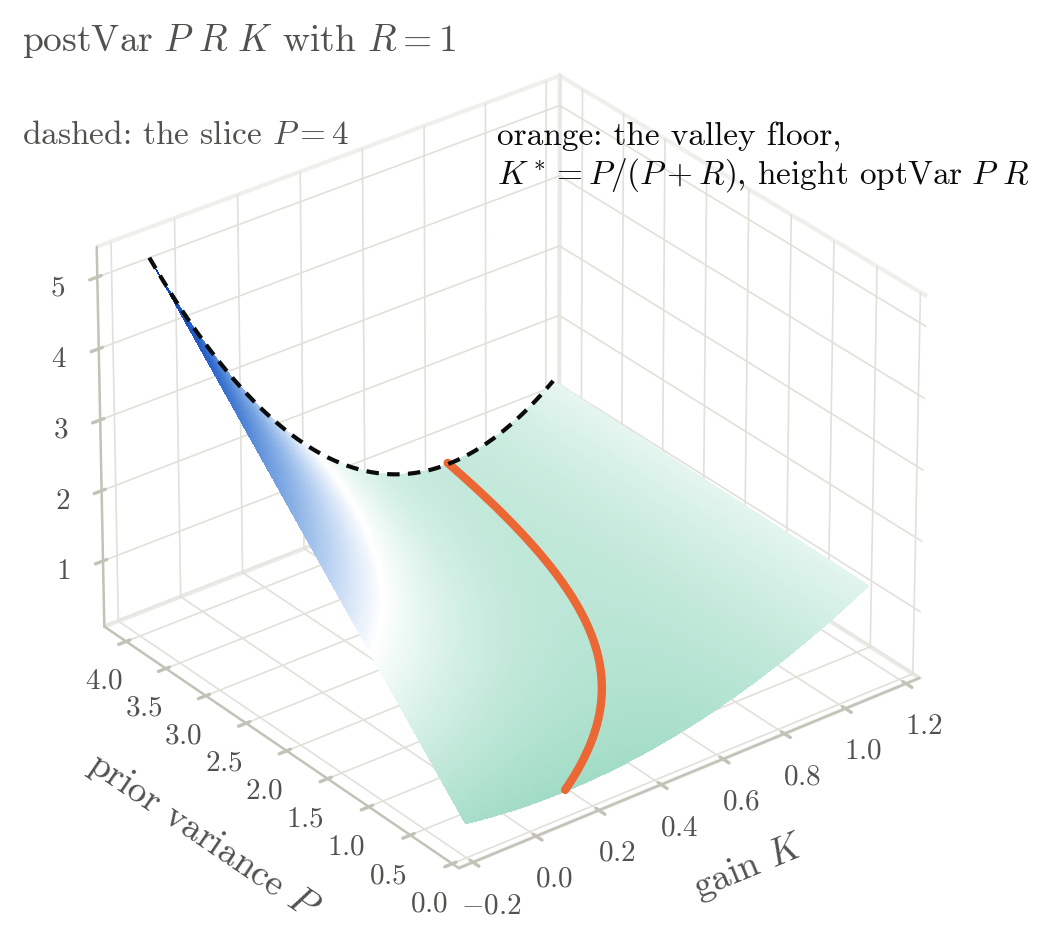
\includegraphics[width=0.6\linewidth]{figures/valley.png}
  \caption{The update variance $\postVar(P, R, K)$ for $R = 1$, over the gain $K$ and the
    prior variance $P$. For every $P$ the minimum over $K$ (orange) sits at $K^* = P/(P + R)$
    with height $\optVar(P, R)$; the dashed parabola is the slice $P = 4$.}
  \label{fig:valley}
\end{figure}

\subsection*{Predict}

Push the guess through one OU step \eqref{eq:ou}: the next prediction is $a\,m$, and its error
variance is $a^2\,\optVar(P, R) + Q$. Combining the two halves gives a recursion for the
variance $P_n$ just before the $n$-th reading, called the \emph{Riccati recursion}:
\begin{equation}\label{eq:riccati}
  P_{n+1} = a^2\,\frac{P_n R}{P_n + R} + Q .
\end{equation}
This is the Lean definition \lean{riccatiStep}, and \lean{riccatiIter} iterates it from a
start $P_0$. It does not depend on the readings, only on $a$, $Q$ and $R$; for an OU mode
started at equilibrium ($P_0 = \sigma^2$, $Q = \sigma^2(1 - a^2)$) it is \lean{ouRiccati}.
Figure~\ref{fig:run} shows the filter at work, and Figure~\ref{fig:riccati} shows that runs of
\eqref{eq:riccati} from different starts all meet at one fixed point $P_\infty$.

\begin{figure}[htbp]
  \centering
  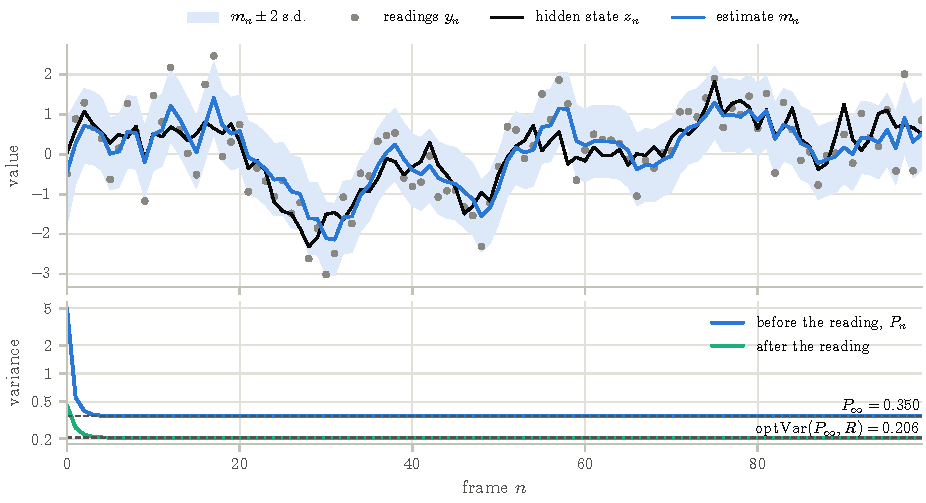
\includegraphics[width=\figwidth]{figures/filter_run.pdf}
  \caption{The filter on a simulated OU mode ($a = \val{runA}$, $Q = \val{runQ}$,
    $R = \val{runR}$), started deliberately unsure ($P_0 = \val{runPzero}$). Top: after frame
    20 the hidden state lies within two standard deviations of the estimate in \val{runIn} of
    \val{runLate} frames. Bottom: the variances before and after each reading settle within a
    few frames.}
  \label{fig:run}
\end{figure}

\begin{figure}[htbp]
  \centering
  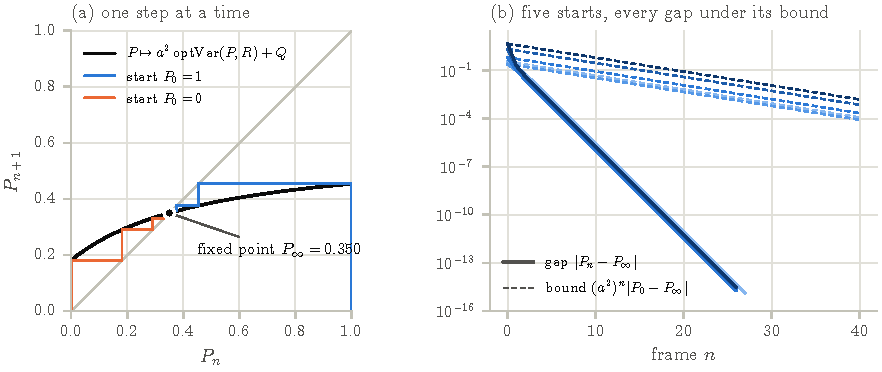
\includegraphics[width=\figwidth]{figures/riccati.pdf}
  \caption{The recursion \eqref{eq:riccati} for the mode of Figure~\ref{fig:run}. (a) Cobweb:
    each step goes up to the curve and across to the diagonal; both starts end at the fixed
    point. (b) The gap to the fixed point shrinks at least as fast as $(a^2)^n$, with
    $a^2 = \val{rAsq}$ (dashed). Near $P_\infty$ it actually shrinks by about \val{rSlope} per
    frame, and the largest ratio of gap to bound is \val{rWorst}.}
  \label{fig:riccati}
\end{figure}

\intuition{trust each source in proportion to its precision, then let the dynamics blur the
  result a little.}

\section{Innovations: the filter's surprises}\label{sec:innovations}

The \emph{innovation} is the part of a reading the filter did not predict:
\[
  \nu_n = y_n - m^-_n = e_n + v_n .
\]
If the model is right and the gain is the Kalman gain, then $\Var(\nu_n) = S_n = P_n + R$, and
innovations at different frames are uncorrelated, or \emph{white}. Both can be checked on
data, channel by channel:
\begin{itemize}
  \item \textbf{Size:} is the measured variance of the innovations, divided by $S$, close
    to 1?
  \item \textbf{Pattern:} is their autocorrelation close to 0 at every lag $k \ge 1$?
\end{itemize}
In the research run, a backbone torsion was deliberately hidden from the model, and one
channel's innovations came out at about 4 times their expected level. The next section
explains exactly what such a ratio means.

\intuition{a good model is surprised by the right amount, and never in a predictable way.}

\section{Two ways the model can be wrong, and their fingerprints}\label{sec:fingerprints}

\textbf{An omitted coordinate (size).} Suppose a channel's reading also contains a coordinate
$h$ that the model leaves out, independent of $e$ and $v$, with $\Var(h) = \tau^2$. Then
$\nu = e + v + h$ and
\[
  \frac{\Var(\nu)}{S} = \frac{S + \tau^2}{S} = 1 + \frac{\tau^2}{S}.
\]
The observed 4x therefore means $\tau^2 \approx 3S$: the hidden torsion carried three times
the variance the filter expected (Figure~\ref{fig:diag}a).

\textbf{A hidden switch (pattern).} Suppose instead the filter ignores the basin label. For two
basins the label is a Markov chain with transition matrix
\[
  M = \begin{pmatrix} 1 - p & p \\ q & 1 - q \end{pmatrix},
\]
where $p$ and $q$ are the switching probabilities per frame (Figure~\ref{fig:twostate}). Its
eigenvalues are $1$ and $\lambda = 1 - p - q$, and $(p, -q)$ is an eigenvector for $\lambda$.
Read as a function on the two states, $f(A) = p$ and $f(B) = -q$, this says
$\Ex[f(s_{n+1}) \mid s_n] = \lambda f(s_n)$: the label's deviation from equilibrium shrinks by
$\lambda$ per frame. When switches are rare, $\lambda$ is close to 1 and the label has a long
memory. A filter that ignores the switch passes this memory into its innovations. The research
model takes their lag covariances $c_n$ to follow
\[
  c_{n+1} = \alpha\,c_n + \beta\,\lambda^{n+1},
\]
where $\alpha = a(1 - K)$ is the filter's own decay per frame and $\beta$ measures how strongly
the switch leaks in. If $|\alpha| < |\lambda|$, then $c_{n+1}/c_n \to \lambda$: the tail of
the autocorrelation decays at the switch's rate (Figure~\ref{fig:diag}b).

\begin{figure}[htbp]
  \centering
  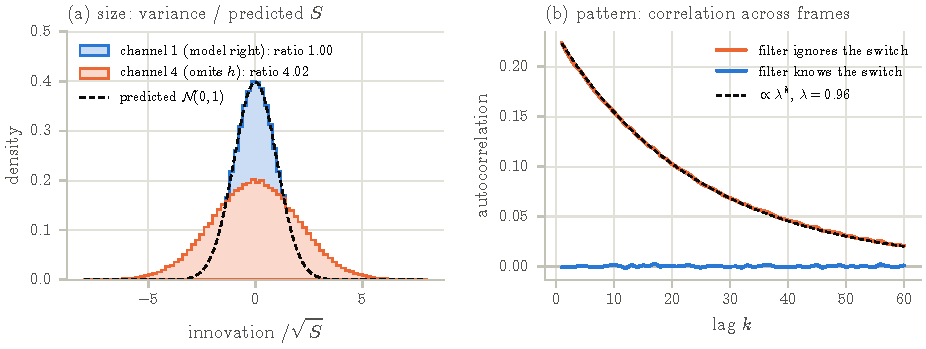
\includegraphics[width=\figwidth]{figures/diagnostics.pdf}
  \caption{The two innovation tests on simulated data. (a) Size: with $\tau^2 = 3S$, channel
    \val{dFlag} has variance ratio \val{dRatioBad} against the theory value 4; a correctly
    modeled channel gives \val{dRatioOk} (\val{dN} innovations each). (b) Pattern: a filter
    that ignores a two-state switch ($p = q = 0.02$, \val{dNac} frames) leaves correlations
    that decay like $\lambda^k$; a fit gives $\hat\lambda = \val{dLamHat}$ against
    $\lambda = \val{dLam}$. With the switch known, no lag exceeds \val{dRhoMax}.}
  \label{fig:diag}
\end{figure}

\begin{figure}[htbp]
  \centering
  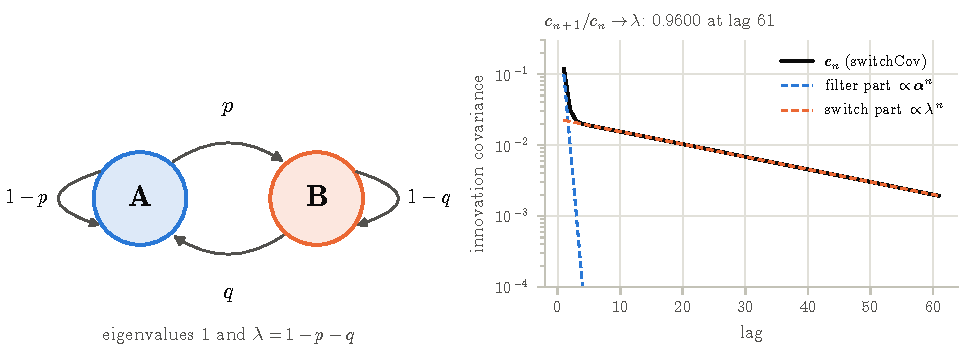
\includegraphics[width=\figwidth]{figures/two_state.pdf}
  \caption{Left: the two-state switch with switching probabilities $p$ and $q$ per frame.
    Right: the lag covariances $c_n$ (\lean{switchCov}) for $\alpha = \val{hAlpha}$,
    $\lambda = \val{hLam}$: a fast filter part $\propto \alpha^n$ dies within a few lags, and
    the switch part $\propto \lambda^n$ sets the tail, so $c_{n+1}/c_n \to \lambda$.}
  \label{fig:twostate}
\end{figure}

\intuition{surprises that are too large point to a missing coordinate; correlations that fade
  slowly point to a hidden switch.}

% =======================================================================================
\partheading{II}{What should be proved, and what is assumed}

\section{The verification agenda}

Part~I gives a model and a procedure. Before trusting a diagnosis made with them, one wants
guarantees. Table~\ref{tab:agenda} lists the questions, why each matters for an MD study, and
the Lean result that answers it; Part~III states each result exactly.

\begin{table}[htbp]
  \centering\small
  \begin{tabularx}{\linewidth}{@{}>{\raggedright}p{0.36\linewidth}>{\raggedright}X l@{}}
    \toprule
    \textbf{Question} & \textbf{Why it matters} & \textbf{Result} \tabularnewline
    \midrule
    Is the Kalman update the best linear blend, and the only best one?
      & the filter's core step is right & Core \tabularnewline
    Does the blend beat both of its sources?
      & a reading never makes the estimate worse & Core \tabularnewline
    Can coordinate families be fused in any order, and does each help?
      & the answer cannot depend on bookkeeping & S \tabularnewline
    Can tracking an OU mode be worse than knowing only its spread?
      & the filter never loses track of a basin & O \tabularnewline
    Is \eqref{eq:postvar} a theorem about random variables?
      & links the algebra to probability & A \tabularnewline
    Exactly how much does an omitted coordinate inflate the innovations?
      & turns the observed 4x into the size of what is missing & D, F5 \tabularnewline
    Are white innovations a sure sign of the right gain?
      & then any pattern proves the gain or the model wrong & W \tabularnewline
    What fingerprint does a hidden switch leave?
      & identifies a missing basin from data & H0, H \tabularnewline
    Does the jump rule keep the intended populations?
      & the surrogate has the right equilibrium & M \tabularnewline
    Does the filter forget its start, settle, and stay calibrated?
      & justifies a burn-in and a single reference level & F \tabularnewline
    \bottomrule
  \end{tabularx}
  \caption{What is worth proving about the model and the filter.}
  \label{tab:agenda}
\end{table}

\intuition{prove the steps a diagnosis relies on, so that only the data can be wrong.}

\section{Assumptions: what the theorems take as given}

A theorem turns assumptions into conclusions; the data must still support the assumptions.
Table~\ref{tab:assume} lists each one, the results that use it, and a way to check it on an
MD run.

\begin{table}[htbp]
  \centering\small
  \begin{tabularx}{\linewidth}{@{}>{\raggedright}X l >{\raggedright}X@{}}
    \toprule
    \textbf{Assumption} & \textbf{Used by} & \textbf{Empirical check} \tabularnewline
    \midrule
    Each slow mode is linear-Gaussian (OU) with constant $a$ and $Q$
      & O, F & each slow coordinate's autocorrelation decays like $a^n$; residuals look
      Gaussian \tabularnewline
    Sensor noise is independent of the state error and across channels
      & A, D, F5 & cross-correlations of innovations between channels are near 0
      \tabularnewline
    Each channel's noise variance $R$ is known and constant
      & F, W, D & channels without an omitted coordinate show ratios near 1
      (Figure~\ref{fig:diag}a) \tabularnewline
    The filter has reached its steady state
      & W, F5 & burn-in discarded (Section~\ref{sec:practice}); $P_n$ flat afterwards
      \tabularnewline
    Jump rates follow the square-root rule at a fixed slow state
      & M & transition counts give $p_i k_{ij} \approx p_j k_{ji}$
      (Section~\ref{sec:equilibrium}) \tabularnewline
    The switch is a constant-rate two-state chain
      & H0, H & dwell times in each basin are exponentially distributed \tabularnewline
    \bottomrule
  \end{tabularx}
  \caption{The assumptions behind the results, and how to test each on data.}
  \label{tab:assume}
\end{table}

Four modeling simplifications deserve to be stated plainly.
\begin{itemize}
  \item \textbf{Second moments only.} The recursions \lean{ouRiccati}, \lean{riccatiIter},
    \lean{innovCov} and \lean{switchCov} are definitions of variances and covariances; Lean
    does not derive them from a stochastic process. Only A, D and F5 are proved from random
    variables.
  \item \textbf{Scalar.} One mode and one sensor at a time; no vectors or matrices of states.
  \item \textbf{Linear-optimal.} $K^*$ is the best \emph{linear} update for any errors with
    the given variances. It is the best of all estimators only for Gaussian errors; heavy
    tails or several modes break that.
  \item \textbf{Approximate switch.} H uses the constant-rate two-state approximation of the
    switch, not the state-dependent rule \eqref{eq:jump}; M holds at one fixed slow state.
\end{itemize}

\intuition{the theorems are exact; whether they apply is a question for the data.}

\section{What the theorems give an MD run}\label{sec:practice}

\begin{itemize}
  \item \textbf{Burn-in.} With frame spacing $\Delta t$ and relaxation time $\tau_c$,
    $a = e^{-\Delta t/\tau_c}$, so by F the influence of the starting variance shrinks at
    least like $(a^2)^n = e^{-2n\Delta t/\tau_c}$. To shrink it below a fraction
    $\varepsilon$, discard
    \[
      n \ge \frac{\tau_c}{2\Delta t}\,\ln\frac{1}{\varepsilon}
    \]
    frames: \val{burnTwo} frames for $\varepsilon = 10^{-2}$ and \val{burnThree} for
    $\varepsilon = 10^{-3}$ when $\tau_c = 10\,\Delta t$ (Figure~\ref{fig:practice}a).
  \item \textbf{Reference level.} After burn-in, each channel's innovations should have
    variance $S_\infty = P_\infty + R$, where $P_\infty$ is \lean{steadyVar}.
  \item \textbf{Detectability.} An omitted coordinate gives exactly $1 + \tau^2/S_\infty$
    (F5). With $N$ white innovations the measured ratio fluctuates by about $\sqrt{2/N}$
    (standard sampling theory, not proved in Lean), so an excess above $3\sqrt{2/N}$ stands
    out: \val{thrK} for $N = 1{,}000$ and \val{thrH} for $N = 100{,}000$
    (Figure~\ref{fig:practice}b).
\end{itemize}

\begin{figure}[htbp]
  \centering
  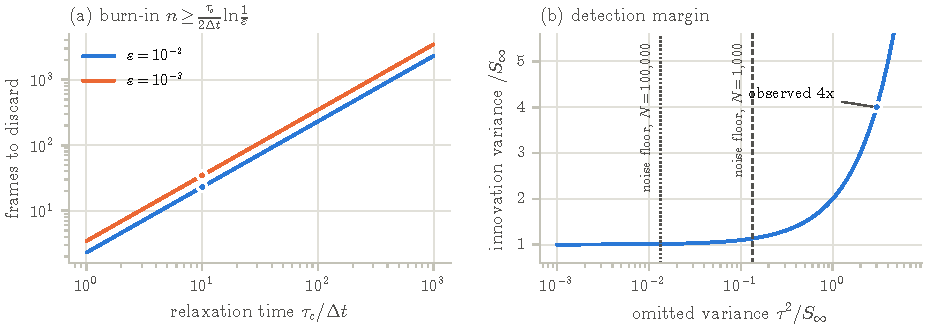
\includegraphics[width=\figwidth]{figures/practice.pdf}
  \caption{(a) Frames to discard before the start is forgotten, against the relaxation time.
    (b) The exact margin $1 + \tau^2/S_\infty$ of F5 against two sampling noise floors; the
    observed 4x is far above both.}
  \label{fig:practice}
\end{figure}

\intuition{discard the burn-in, then judge each channel against $S_\infty$, above the noise
  floor.}

% =======================================================================================
\partheading{III}{The model in Lean}

\section{Lean in five minutes}

\begin{itemize}
  \item \textbf{What Lean does.} Lean is a programming language and a proof assistant. You
    write definitions, statements and proofs. A small trusted core, the \emph{kernel}, checks
    every step of every proof; a proof is either accepted or rejected. \emph{Mathlib} is
    Lean's mathematics library: real numbers, limits, matrices, probability.
  \item \textbf{What Lean does not do.} It checks that a proof proves the statement, not that
    the statement says what you meant. So the definitions and the final statements are read
    and approved by a person; the rest is left to the kernel.
  \item \textbf{Reading a statement.} \lean{theorem name (P R : ℝ) (hP : 0 ≤ P) (hR : 0 < R) :
    C} means: for all real $P$ and $R$ with $0 \le P$ and $0 < R$, the claim $C$ holds. The
    hypotheses have names (\lean{hP}, \lean{hR}) so that the proof can use them. Functions are
    applied without brackets: \lean{gain P R} is $\mathrm{gain}(P, R)$.
  \item \textbf{Division is total.} In Lean $x / 0 = 0$, so \lean{gain P R = P / (P + R)} is
    defined even when $P + R = 0$. That is why the theorems carry hypotheses such as $0 < R$.
  \item \textbf{Axioms.} Lean and Mathlib use three standard axioms: propositional
    extensionality (\lean{propext}), the axiom of choice (\lean{Classical.choice}) and
    quotient soundness (\lean{Quot.sound}). The command \lean{\#print axioms} lists what a
    theorem depends on. An unfinished proof would show up there as \lean{sorryAx}.
\end{itemize}

Table~\ref{tab:rosetta} translates the notation that appears below.

\begin{table}[htbp]
  \centering\small
  \begin{tabularx}{\linewidth}{@{}>{\raggedright}p{0.42\linewidth}>{\raggedright\arraybackslash}X@{}}
    \toprule
    \textbf{Lean} & \textbf{Mathematics} \\
    \midrule
    \lean{ℝ}, \lean{ℕ} & the real numbers; the natural numbers $0, 1, 2, \dots$ \\
    \lean{a \textasciicircum{} 2}, \lean{|x|}, \lean{Real.sqrt x} & $a^2$, $|x|$, $\sqrt{x}$ \\
    \lean{∀ x, A};\enspace \lean{A → B};\enspace \lean{A ∧ B};\enspace \lean{A ↔ B}
      & for all $x$, $A$; if $A$ then $B$; $A$ and $B$; $A$ if and only if $B$ \\
    \lean{| 0 => u0 | n + 1 => g (u n)} & the sequence $u_0$, $u_{n+1} = g(u_n)$ \\
    \lean{Tendsto u atTop (𝓝 L)} & $u_n \to L$ as $n \to \infty$ \\
    \lean{Fin n};\enspace \lean{Matrix (Fin n) (Fin n) ℝ}
      & the indices $\{0, \dots, n-1\}$; real $n \times n$ matrices \\
    \lean{!![a, b; c, d]};\enspace \lean{![u, v]}
      & the matrix with rows $(a, b)$ and $(c, d)$; the vector $(u, v)$ \\
    \lean{M.mulVec v};\enspace \lean{Matrix.vecMul p L} & $M v$; $p^\transp L$ \\
    \lean{∑ k ∈ Finset.univ.erase i, f k} & $\sum_{k \ne i} f(k)$ \\
    \lean{Ω}, \lean{μ}, \lean{[IsProbabilityMeasure μ]} & a probability space \\
    \lean{e : Ω → ℝ} & a random variable $e$ \\
    \lean{MemLp e 2 μ} & $\Ex[e^2] < \infty$, so $e$ has a variance \\
    \lean{IndepFun e v μ} & $e$ and $v$ are independent \\
    \lean{variance e μ};\enspace \lean{c • e} & $\Var(e)$; the random variable $c\,e$ \\
    \bottomrule
  \end{tabularx}
  \caption{Reading Lean notation.}
  \label{tab:rosetta}
\end{table}

\intuition{Lean guarantees that each proof matches its statement, not that the statement
  matches your idea.}

\section{The file and its trust boundary}

All the Lean work is in one file, \lean{Kalman.lean}, divided into Parts
(Figure~\ref{fig:leanfile}). Parts 1 and 3 hold the \val{nDefsCore} core and \val{nDefsModel}
model definitions, and Part~6 the \val{nSpec} final statements: these are what a person reads.
Parts 2, 4, 4b, 4c and 5 hold \val{nProofs} proofs, which Lean checks. Each Part~6 theorem is
proved in one line by citing a lemma from a proof Part. Part~1 and the six proofs of Part~2
are the student's own work, copied unchanged from \lean{Core.lean}.

The trust argument is short. Suppose that (1) the definitions of Parts 1 and 3 mean what
Part~I says, (2) each Part~6 statement says what Section~\ref{sec:statements} says it says,
and (3) Lean accepts the file and \lean{\#print axioms} lists only the three standard axioms.
Then every statement is true. Lean guarantees (3); Sections~\ref{sec:defs}
and~\ref{sec:statements} are there to help you check (1) and (2).

\begin{figure}[htbp]
  \centering
  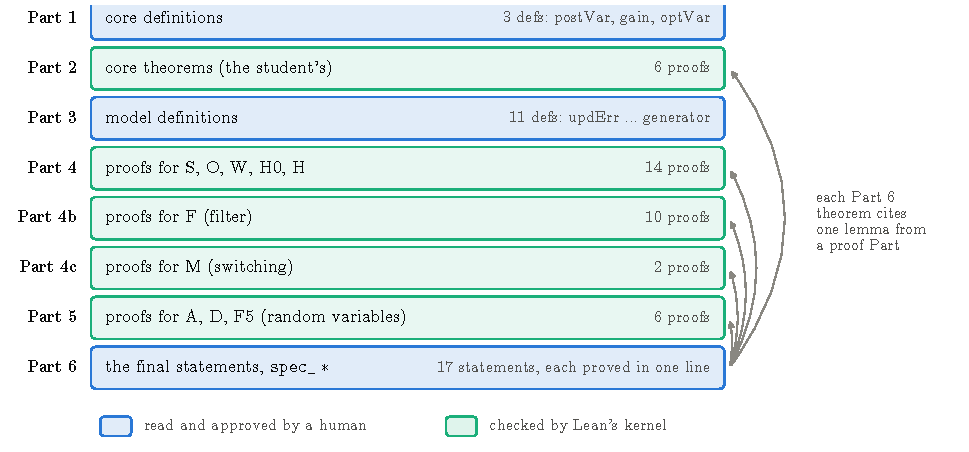
\includegraphics[width=\figwidth]{figures/lean_file.pdf}
  \caption{The Parts of \lean{Kalman.lean}. Blue Parts are read and approved by a person,
    green Parts are checked by Lean's kernel; each final statement in Part~6 cites one lemma
    from a green Part.}
  \label{fig:leanfile}
\end{figure}

\intuition{read the blue Parts; the kernel checks the green ones.}

\section{The definitions}\label{sec:defs}

Each excerpt below is copied verbatim from \lean{Kalman.lean} by the figure script, so what you
read is exactly what Lean checks. Two index conventions: \lean{Fin n} counts from 0, and the
sequences \lean{innovCov} and \lean{switchCov} start at lag~1, so index $k$ holds lag $k + 1$.

\subsection*{Part 1: the core update (the student's)}

\leanfile{postVar}
The variance \eqref{eq:postvar} of the update error $(1 - K)e - Kv$, when $\Var e = P$ and
$\Var v = R$.

\leanfile{gain}
The Kalman gain $K^* = P/(P + R)$.

\leanfile{optVar}
The smallest update variance $PR/(P + R)$, reached at $K = K^*$.

\subsection*{Part 3: the model}

\leanfile{updErr}
The update error as a random variable: a function on the sample space $\Omega$, sending each
outcome $\omega$ to $(1 - K)\,e(\omega) - K\,v(\omega)$.

\leanfile{ouPredict}
One OU prediction step for a variance: $P \mapsto a^2 P + \sigma^2(1 - a^2)$
(Section~\ref{sec:ou}). Lean's \lean{σ2} is the equilibrium variance $\sigma^2$.

\leanfile{ouRiccati}
The prior variance of an OU mode under the optimal filter, started at equilibrium:
\[
  P_0 = \sigma^2, \qquad P_{n+1} = \mathrm{ouPredict}\bigl(\optVar(P_n, R)\bigr),
\]
that is \eqref{eq:riccati} with $Q = \sigma^2(1 - a^2)$.

\leanfile{innovCov}
Innovation autocovariances at steady state for a gain $K$: lag~1 is $a(1 - K)P - aKR$, and each
further lag multiplies by the filter's decay $a(1 - K)$.

\leanfile{msm}
The two-state transition matrix $M = \left(\begin{smallmatrix} 1-p & p \\ q & 1-q
\end{smallmatrix}\right)$ (a Markov state model, MSM).

\leanfile{switchCov}
Lag covariances when a hidden switch leaks in. Writing $c_n$ for the value at index $n$ (lag
$n + 1$): $c_0 = \gamma$, the lag-1 value that Lean calls \lean{c₁}, and
$c_{n+1} = \alpha\,c_n + \beta\,\lambda^{n+1}$ (Section~\ref{sec:fingerprints}).

\leanfile{riccatiStep}
One step of the variance recursion \eqref{eq:riccati}: update with noise $R$, then predict
with decay $a$ and process noise $Q$.

\leanfile{riccatiIter}
The recursion run for $n$ steps from $P_0$.

\leanfile{steadyVar}
The candidate steady state $P_\infty$. A fixed point $P = a^2 PR/(P + R) + Q$ with $P + R > 0$
satisfies $P^2 + (R(1 - a^2) - Q)\,P - QR = 0$; \lean{steadyVar} is the root with the plus
sign.

\leanfile{jumpRate}
The jump rule \eqref{eq:jump}: $k_{ij} = \kappa_{ij}\sqrt{p_j/p_i}$.

\leanfile{generator}
The generator $L$ of Section~\ref{sec:surrogate}: jump rates off the diagonal, and minus each
row's total outflow on the diagonal.

\section{The seventeen verified statements}\label{sec:statements}

Each statement is shown as it appears in Part~6, without its one-line proof. Below each one:
what it says, and what it means for the model.

\subsection{Core: the Kalman update}

\leanfile{spec_gain_optimal}
\reads{for all real $P, R, K$ with $P \ge 0$ and $R > 0$:
  $\postVar(P, R, K^*) \le \postVar(P, R, K)$.}
  {no gain gives a smaller error variance after a reading than the Kalman gain.}

\leanfile{spec_gain_unique}
\reads{if moreover $\postVar(P, R, K) = \postVar(P, R, K^*)$, then $K = K^*$.}
  {the best gain is unique, so ``the'' Kalman gain is well defined.}

\leanfile{spec_optVar_le}
\reads{$\optVar(P, R) \le P$ and $\optVar(P, R) \le R$.}
  {after an update, the error is smaller than both the prediction's and the reading's.}

\subsection{S: sensor fusion}

\leanfile{spec_fusion_comm}
\reads{for $P \ge 0$ and $R_1, R_2 > 0$:
  $\optVar(\optVar(P, R_1), R_2) = \optVar(\optVar(P, R_2), R_1)$.}
  {fusing two coordinate families gives the same variance in either order.}

\leanfile{spec_fusion_mono}
\reads{$\optVar(\optVar(P, R_1), R_2) \le \optVar(P, R_1)$.}
  {each additional coordinate family can only help.}

\subsection{O: an OU mode stays within its equilibrium spread}

\leanfile{spec_ou_bound}
\reads{if $a^2 \le 1$, $\sigma^2 \ge 0$ and $R > 0$, then every term $P_n$ of
  \lean{ouRiccati} satisfies $0 \le P_n \le \sigma^2$.}
  {filtering an OU mode is never worse than knowing only its equilibrium spread.}

\subsection{A: the variance formula from random variables}

\leanfile{spec_variance_update}
\reads{on a probability space, if $e$ and $v$ are independent and have variances, then for
  every $K$: $\Var((1 - K)e - Kv) = \postVar(\Var e, \Var v, K)$.}
  {formula \eqref{eq:postvar} is a theorem about random variables, not an assumption.}

\leanfile{spec_variance_update_optimal}
\reads{if moreover $\Var v > 0$, the gain $\Var e / (\Var e + \Var v)$ gives the update error
  with the smallest variance.}
  {the Kalman gain is optimal for the actual random errors.}

\subsection{D: an omitted coordinate}

\leanfile{spec_innov_excess}
\reads{if $e, v, h$ have variances, $e$ is independent of $v$, and $e + v$ is independent of
  $h$: $\Var(e + v + h) = (\Var e + \Var v) + \Var h$.}
  {an omitted coordinate adds its whole variance to the innovations.}

\leanfile{spec_innov_excess_ratio}
\reads{if also $S = \Var e + \Var v > 0$ and $\Var h > 0$: $\Var(e + v + h)/S > 1$.}
  {any omitted coordinate with nonzero variance pushes the innovation ratio above 1.}

\subsection{W: white innovations}

\leanfile{spec_white_iff}
\reads{for $a \ne 0$, $P \ge 0$ and $R > 0$: every lag of \lean{innovCov} is $0$ if and only
  if $K = P/(P + R)$.}
  {white innovations occur exactly at the Kalman gain, so any correlation means a wrong gain
  or a wrong model.}

\subsection{H0 and H: the hidden switch}

\leanfile{spec_msm_eigen}
\reads{for all real $p, q$: $M\,(p, -q)^\transp = (1 - p - q)\,(p, -q)^\transp$.}
  {a deviation from the switch's equilibrium shrinks by $\lambda = 1 - p - q$ per frame.}

\leanfile{spec_switch_ratio}
\reads{if $\beta \ne 0$ and $|\alpha| < |\lambda|$, the lag covariances of \lean{switchCov}
  satisfy $c_{n+1}/c_n \to \lambda$ as $n \to \infty$.}
  {the slow tail of the innovations' autocovariance reveals the switch's eigenvalue.}

\subsection{M: the switching keeps its equilibrium}

\leanfile{spec_detailed_balance}
\reads{for $p_i, p_j > 0$ and every $\kappa$:
  $p_i \cdot \mathrm{jumpRate}(\kappa, p_i, p_j) = p_j \cdot \mathrm{jumpRate}(\kappa, p_j,
  p_i)$.}
  {the square-root rule balances the flow between every pair of basins.}

\leanfile{spec_populations_stationary}
\reads{if $\kappa_{ij} = \kappa_{ji}$ for all $i, j$ and every $p_i > 0$, then $p^\transp L = 0$
  for $L = \mathrm{generator}(\kappa, p)$.}
  {started at the target populations, the switching stays there: the surrogate keeps its
  equilibrium.}

\subsection{F: the filter forgets its start, converges, and is calibrated}

\leanfile{spec_filter_guarantee}
\reads{if $a^2 < 1$, $a \ne 0$, $Q \ge 0$ and $R > 0$, then: (1) for all starts
  $P_0, P_0' \ge 0$ and all $n$, the two runs of \eqref{eq:riccati} satisfy
  $|P_n - P_n'| \le (a^2)^n |P_0 - P_0'|$; (2) $P_\infty = \mathrm{steadyVar}(a, Q, R)$ is
  nonnegative and a fixed point; (3) every run with $P_0 \ge 0$ tends to $P_\infty$; (4) at
  $P_\infty$ with the Kalman gain, every innovation autocovariance is $0$.}
  {the filter forgets how it was started, settles to one steady state, and is calibrated
  there.}

\subsection{F5: the exact detection margin}

\leanfile{spec_detection_margin}
\reads{under the hypotheses of D with $S = \Var e + \Var v > 0$:
  $\Var(e + v + h)/S = 1 + \Var(h)/S$.}
  {the innovation ratio measures the omitted variance exactly: 4x means $\Var h = 3S$.}

\section{The verification record}\label{sec:record}

The file is built with \lean{lake build LoVe.Final\_Project.Kalman} on Lean and Mathlib
v4.33.0. The build ends with ``Build completed successfully'', with no errors, no warnings and
no \lean{sorry}. A search of the file for \lean{sorry}, \lean{admit} and \lean{native\_decide}
finds nothing, and the file declares no axioms. The \lean{\#print axioms} line for each of the
\val{nSpec} statements reports (with the file-and-line prefixes removed):

\begin{tcolorbox}[enhanced, colback=wash, colframe=wash, boxrule=0pt, arc=2pt, left=4pt,
    right=4pt, top=2pt, bottom=2pt]
  \VerbatimInput[fontsize=\leancodesize]{build_record.txt}
\end{tcolorbox}

Finally, a script compared the definitions and statements against their sources: Part~1
matches the student's \lean{Core.lean}, and Parts 3 and 6 match the definitions and statements
supplied for the project, character for character.

\intuition{a clean build with only the three standard axioms means every statement above is
  proved.}

% =======================================================================================
\appendix
\phantomsection
\addcontentsline{toc}{part}{Appendices}

\section{How each result is proved}\label{app:proofs}

Each proof below is a short paper argument, followed by the chain of Lean lemmas that carries
it out. All the lemmas are in \lean{Kalman.lean}; the Mathlib facts they use are listed in
Appendix~\ref{app:mathlib}.

\subsection{Core: complete the square}

The key identity is \eqref{eq:square}. In Lean, \lean{complete\_square} unfolds the
definitions, clears the denominator $P + R > 0$ (\lean{denom\_pos}) with \lean{field\_simp}, and
finishes with \lean{ring}; \lean{postVar\_gain} shows $\postVar(P, R, K^*) = \optVar(P, R)$.
Then:
\begin{itemize}
  \item \textbf{Optimal.} After rewriting with both identities, the claim is
    $\optVar \le (P + R)(K - K^*)^2 + \optVar$, a product of a positive number and a square.
  \item \textbf{Unique.} Equal variances force $(P + R)(K - K^*)^2 = 0$. Since $P + R \ne 0$,
    the square is $0$, so $K = K^*$.
  \item \textbf{Beats both sources.} Clearing the denominator, $\optVar \le P$ becomes
    $PR \le P(P + R)$, true since $R \le P + R$ and $P \ge 0$; and $\optVar \le R$ becomes
    $PR \le R(P + R)$, which \lean{nlinarith} proves.
\end{itemize}
The student's proof of optimality, verbatim:
\leanfile{gain_optimal}

\subsection{S: sensor fusion}

Both fusion orders simplify to $P R_1 R_2 / (P R_1 + P R_2 + R_1 R_2)$
(\lean{optVar\_optVar}: \lean{field\_simp}, then \lean{ring}), which is symmetric in $R_1$
and $R_2$. Monotonicity is \lean{optVar\_le} applied to the prior $\optVar(P, R_1) \ge 0$.

\subsection{O: the OU bound}

Induction on $n$, proving both bounds at once. If $0 \le x \le \sigma^2$, the update gives
$0 \le \optVar(x, R) \le x \le \sigma^2$, and the prediction
$a^2 y + \sigma^2(1 - a^2)$ is a weighted average of $y \in [0, \sigma^2]$ and $\sigma^2$ with
weights $a^2$ and $1 - a^2$ in $[0, 1]$, so it stays in $[0, \sigma^2]$
(\lean{ouPredict\_mem}, a \lean{calc} chain with \lean{gcongr}; then \lean{ou\_bound}).

\subsection{A: the variance formula}

Write the update error as $(1 - K)\cdot e + (-K)\cdot v$ (\lean{updErr\_eq}). Scaled copies of
independent variables are independent (\lean{IndepFun.comp}), so the sum rule
(\lean{IndepFun.variance\_add}) and the scaling rule (\lean{variance\_smul}) give
$(1 - K)^2\Var e + K^2\Var v$. Optimality then follows from \lean{gain\_optimal} with
$P = \Var e \ge 0$ and $R = \Var v > 0$.
\leanfile{variance_update}

\subsection{D and F5: the omitted coordinate}

Apply the sum rule to $(e + v) + h$, then to $e + v$ (\lean{innov\_excess}). The ratio exceeds
1 because $S < S + \Var h$ and $S > 0$ (\lean{one\_lt\_div}). For the exact margin, rewrite the
numerator with \lean{innov\_excess}; then $(S + \tau^2)/S = 1 + \tau^2/S$ because $S \ne 0$
(\lean{add\_div}, \lean{div\_self}).

\subsection{W: white innovations}

By induction, lag $k + 1$ is $(a(1 - K))^k$ times lag 1 (\lean{innovCov\_closed}), and lag 1
equals $a\,(P + R)\,(K^* - K)$ (\lean{innovCov\_zero}). If every lag vanishes, lag 1 does, so
$K = K^*$ because $a \ne 0$ and $P + R > 0$. Conversely, at $K = K^*$ lag 1 is 0, hence every
lag is 0.
\leanfile{white_iff}

\subsection{H0: the switch's eigenvector}

Compute both entries of $M\,(p, -q)^\transp$: $(1 - p)p - pq = p(1 - p - q)$ and
$qp - (1 - q)q = -q(1 - p - q)$. In Lean: split into the two entries (\lean{fin\_cases}),
unfold with \lean{simp}, finish with \lean{ring}.

\subsection{H: the switch's decay rate}

From $|\alpha| < |\lambda|$ we get $\lambda \ne 0$ and $\lambda \ne \alpha$ (\lean{lam\_ne}).
Induction gives the closed form $c_n = (\gamma - B)\,\alpha^n + B\,\lambda^n$ with
$B = \beta\lambda/(\lambda - \alpha)$ and $\gamma = c_0$ (\lean{switchCov\_closed}). Dividing
by $\lambda^n$, $c_n/\lambda^n = (\gamma - B)(\alpha/\lambda)^n + B \to B$ since
$|\alpha/\lambda| < 1$
(\lean{switchCov\_div\_tendsto}). Finally
$c_{n+1}/c_n = \lambda \cdot \dfrac{c_{n+1}/\lambda^{n+1}}{c_n/\lambda^n} \to \lambda \cdot
\dfrac{B}{B} = \lambda$, using $B \ne 0$, which holds because $\beta \ne 0$
(\lean{switch\_ratio}).

\subsection{M: detailed balance and stationary populations}

\textbf{M1.} Split $\sqrt{p_j/p_i} = \sqrt{p_j}/\sqrt{p_i}$ and use $p_i/\sqrt{p_i} =
\sqrt{p_i}$; both sides become $\kappa\sqrt{p_i}\sqrt{p_j}$:
\leanfile{detailed_balance}

\textbf{M2.} Entry $j$ of $p^\transp L$ is $p_j L_{jj} + \sum_{i \ne j} p_i L_{ij}$. By M1 and
$\kappa_{ij} = \kappa_{ji}$, each term $p_i k_{ij}$ equals $p_j k_{ji}$, so the sum is $p_j$
times the total outflow of $j$, which $p_j L_{jj}$ cancels:
\leanfile{populations_stationary}

\subsection{F: the filter guarantee}

\begin{enumerate}
  \item \textbf{Two runs forget their difference.} For $x, y \ge 0$,
    \[
      \optVar(x, R) - \optVar(y, R) = \frac{R^2}{(x + R)(y + R)}\,(x - y),
    \]
    and the factor lies in $[0, 1]$, so $|\optVar(x, R) - \optVar(y, R)| \le |x - y|$
    (\lean{optVar\_lipschitz}). Hence one step of \eqref{eq:riccati} shrinks gaps by $a^2$
    (\lean{riccatiStep\_lipschitz}). The iterates stay $\ge 0$ because $Q \ge 0$
    (\lean{riccatiIter\_nonneg}), and induction gives the $(a^2)^n$ bound
    (\lean{riccati\_contract}).
  \item \textbf{A steady state.} With $D = (R(1 - a^2) - Q)^2 + 4QR \ge (Q - R(1 - a^2))^2$
    we have $\sqrt D \ge |Q - R(1 - a^2)|$, so $P_\infty \ge 0$ (\lean{steadyVar\_nonneg}).
    Squaring the root shows that $P_\infty$ solves the quadratic, which after clearing
    $P_\infty + R > 0$ is the fixed-point equation (\lean{steadyVar\_fixed}).
  \item \textbf{Convergence.} A run started at $P_\infty$ stays there
    (\lean{riccatiIter\_steady}). Comparing any run with that one,
    $|P_n - P_\infty| \le (a^2)^n |P_0 - P_\infty| \to 0$ (\lean{riccati\_tendsto}).
  \item \textbf{Calibration.} The backward direction of W, applied at $P = P_\infty \ge 0$
    (\lean{steady\_white}).
\end{enumerate}
Part (1) holds for every $a$; the hypothesis $a^2 < 1$ is used only in (3), and $a \ne 0$ only
in (4). The convergence proof, verbatim:
\leanfile{riccati_tendsto}

\section{Mathlib facts used}\label{app:mathlib}

\begin{center}\small
  \begin{tabularx}{\linewidth}{@{}>{\raggedright}p{0.5\linewidth}>{\raggedright\arraybackslash}X@{}}
    \toprule
    \textbf{Lemma} & \textbf{Meaning} \\
    \midrule
    \lean{mul\_nonneg}, \lean{sq\_nonneg} & $0 \le a$, $0 \le b \Rightarrow 0 \le ab$;
      $0 \le a^2$ \\
    \lean{le\_add\_iff\_nonneg\_left} & $a \le b + a \iff 0 \le b$ \\
    \lean{add\_eq\_right};\enspace \lean{mul\_eq\_zero}
      & $a + b = b \iff a = 0$;\enspace $ab = 0 \iff a = 0 \lor b = 0$ \\
    \lean{eq\_zero\_of\_pow\_eq\_zero};\enspace \lean{sub\_eq\_zero}
      & $a^n = 0 \Rightarrow a = 0$;\enspace $a - b = 0 \iff a = b$ \\
    \lean{mul\_le\_mul\_of\_nonneg\_left} & $b \le c$, $0 \le a \Rightarrow ab \le ac$ \\
    \lean{div\_le\_one};\enspace \lean{one\_lt\_div}
      & for $0 < b$: $a/b \le 1 \iff a \le b$;\enspace $1 < a/b \iff b < a$ \\
    \lean{abs\_mul};\enspace \lean{abs\_of\_nonneg}
      & $|ab| = |a|\,|b|$;\enspace $0 \le a \Rightarrow |a| = a$ \\
    \lean{mul\_le\_of\_le\_one\_left} & $0 \le b$, $a \le 1 \Rightarrow ab \le b$ \\
    \lean{Real.abs\_le\_sqrt};\enspace \lean{Real.sq\_sqrt}
      & $a^2 \le b \Rightarrow |a| \le \sqrt b$;\enspace $0 \le a \Rightarrow (\sqrt a)^2 = a$ \\
    \lean{Real.sqrt\_div};\enspace \lean{Real.div\_sqrt}
      & $0 \le x \Rightarrow \sqrt{x/y} = \sqrt x/\sqrt y$;\enspace $x/\sqrt x = \sqrt x$ \\
    \lean{tendsto\_pow\_atTop\_nhds\_zero\_of\_lt\_one} & $0 \le r < 1 \Rightarrow r^n \to 0$ \\
    \lean{tendsto\_pow\_atTop\_nhds\_zero\_of\_abs\_lt\_one} & $|r| < 1 \Rightarrow r^n \to 0$ \\
    \lean{squeeze\_zero} & $0 \le u_n \le v_n$ and $v_n \to 0 \Rightarrow u_n \to 0$ \\
    \lean{Finset.add\_sum\_erase};\enspace \lean{Finset.mul\_sum}
      & split one term off a sum;\enspace move a constant factor into a sum \\
    \lean{IndepFun.comp} & functions of independent variables are independent \\
    \lean{IndepFun.variance\_add} & $\Var(X + Y) = \Var X + \Var Y$ for independent $X, Y$ with
      variances \\
    \lean{variance\_smul};\enspace \lean{variance\_nonneg}
      & $\Var(cX) = c^2\Var X$;\enspace $0 \le \Var X$ \\
    \bottomrule
  \end{tabularx}
\end{center}

\section{Symbols}\label{app:symbols}

\begin{center}\small
  \begin{tabularx}{\linewidth}{@{}l>{\raggedright\arraybackslash}X l@{}}
    \toprule
    \textbf{Symbol} & \textbf{Meaning} & \textbf{In Lean} \\
    \midrule
    $V$, $\theta$ & energy landscape; noise strength (temperature) & -- \\
    $p_i$ & population of basin $i$ & \lean{p i}, \lean{pᵢ} \\
    $\kappa_{ij}$, $k_{ij}$ & symmetric prefactor; jump rate $i \to j$ & \lean{κ i j};
      \lean{jumpRate} \\
    $L$ & generator of the basin switching & \lean{generator κ p} \\
    $\tau_c$, $\Delta t$ & relaxation time; frame spacing & -- \\
    $a$, $Q$ & OU decay per frame $e^{-\Delta t/\tau_c}$; process noise & \lean{a}, \lean{Q} \\
    $\sigma^2$ & equilibrium variance of an OU mode & \lean{σ2} \\
    $e$, $v$, $h$ & prediction error; sensor noise; omitted coordinate & \lean{e}, \lean{v},
      \lean{h} \\
    $P$, $R$ & prediction variance $\Var e$; sensor noise variance $\Var v$ & \lean{P},
      \lean{R} \\
    $K$, $K^*$ & a gain; the Kalman gain $P/(P + R)$ & \lean{K}, \lean{gain P R} \\
    $P_n$, $P_\infty$ & prior variance after $n$ frames; its steady state &
      \lean{riccatiIter}, \lean{steadyVar} \\
    $\nu$, $S$ & innovation; its predicted variance $P + R$ & -- \\
    $\tau^2$ & variance of an omitted coordinate & \lean{variance h μ} \\
    $p$, $q$, $\lambda$ & switching probabilities; switch eigenvalue $1 - p - q$ & \lean{p},
      \lean{q}, \lean{lam} \\
    $\alpha$, $\beta$ & filter decay $a(1 - K)$; leak strength of the switch & \lean{α},
      \lean{β} \\
    \bottomrule
  \end{tabularx}
\end{center}

\section{Reproducing everything}\label{app:reproduce}

\begin{itemize}
  \item \textbf{The proofs.} From the repository root (the folder with
    \lean{lakefile.toml}): \lean{lake exe cache get}, then
    \lean{lake build LoVe.Final\_Project.Kalman}.
  \item \textbf{The figures and numbers.} Run \lean{python make\_writeup\_figures.py} in this
    folder. It needs numpy and matplotlib, uses fixed seeds, takes about 5 to 15 minutes, and
    rewrites \lean{figures/}, \lean{generated/numbers.tex} and the verbatim Lean excerpts in
    \lean{generated/lean/}.
  \item \textbf{This document.} Compile \lean{kalman\_writeup.tex} with pdf\LaTeX, Xe\LaTeX,
    Lua\LaTeX\ or Tectonic, twice so the contents settle.
\end{itemize}

\end{document}
